\documentclass[xcolor=table,aspectratio=169]{beamer}
\usetheme{Madrid}
\usepackage{adjustbox}
\usepackage{dcolumn}
\newcolumntype{d}[1]{D{.}{.}{#1}}
%\usetheme{metropolis}
\usepackage[style=verbose-note, sorting=none, sortcites=true, maxnames=1, giveninits=true, autocite=superscript, doi=false, url=false, isbn=false, backend=biber, citetracker=false, pagetracker=false, bibencoding=utf8, eprint=false]{biblatex}
% \usepackage[backend=bibtex,style=authoryear-comp,citestyle=authoryear-comp,firstinits=true,sorting=none,maxnames=1,doi=false,isbn=false,url=false,eprint=false]{biblatex}
\usepackage[T1]{fontenc}
\usepackage[normalem]{ulem}

\definecolor{twitter_blue}{HTML}{1da1f2}
\input{seaborn_colours.tex}

% Gobbling first names

\AtEveryCitekey{%
   \clearfield{shorttitle}%
   \clearfield{month}%
   \clearfield{day}%
   \ifentrytype{article}{%
      \clearfield{title}%
   }{}
   }
\ExecuteBibliographyOptions[online]{eprint=true}

% "blindfootcite" is the equivalent of "footcite" except the number marker does not appear
\newcommand\blfootcite[1]{%
  \begingroup
  \renewcommand\thefootnote{}\footnote{\hspace{-4ex}\cite{#1}}%
  \addtocounter{footnote}{-1}%
  \endgroup
}
% Likewise blfootnote
\newcommand\blfootnote[1]{%
  \begingroup
  \renewcommand\thefootnote{}\footnote{#1}%
  \addtocounter{footnote}{-1}%
  \endgroup
}

\renewcommand*{\multicitedelim}{\textcolor{seaborn_bg_grey_darker}{\addsemicolon}}
\setbeamerfont{footnote}{size=\scriptsize}
\renewcommand\footnoterule{\kern-3pt \color{seaborn_bg_grey_darker}\hrule width \textwidth height 0.4pt \color{black} \kern 2.6pt}

\DeclareSourcemap{
  \maps[datatype=bibtex,overwrite=False]{
   \map{
     \step[fieldsource=journal,
           match={Journal of Chemical Theory and Computation},
           replace={JCTC}]
     \step[fieldsource=journal,
           match={Reviews of Modern Physics},
           replace={Rev. Mod. Phys.}]
     \step[fieldsource=journal,
           match={Reports on Progress in Physics},
           replace={Rep. Prog. Phys.}]
     \step[fieldsource=journal,
           match={Physical Review Letters},
           replace={Phys. Rev. Lett.}]
     \step[fieldsource=journal,
           match={Physical Review},
           replace={Phys. Rev.}]
     \step[fieldsource=journal,
           match={B - Condensed Matter and Materials Physics},
           replace={B}]
     \step[fieldsource=journal,
           match={Journal of Chemical Physics},
           replace={J. Chem. Phys.}]
     \step[fieldsource=journal,
           match={Annual Review of Materials Research},
           replace={Annu. Rev. Mater. Res.}]
   }
  }
}

\renewbibmacro{in:}{}
\DeclareFieldFormat{pages}{\mkfirstpage{#1}}
\beamertemplatenavigationsymbolsempty
\bibliography{references.bib}
\setbeamertemplate{bibliography item}[text]
\renewbibmacro{in:}{}
\AtEveryBibitem{\clearfield{title}}
\AtEveryBibitem{\clearfield{month}}
\AtEveryBibitem{\clearfield{pages}}
\DeclareNameAlias{default}{given-family}

% \renewcommand*{\bibfont}{\tiny}
\usepackage{amssymb}
\usepackage{epsfig}
\usepackage{psfrag}
\usepackage{wrapfig}
\usepackage{graphicx}
\usepackage{color}
\usepackage[table]{xcolor}
\usepackage{amsmath}
\usepackage{multimedia}
\usepackage{subcaption}
%\usepackage{style}
\usepackage{verbatim}
\usepackage{multicol}
\usepackage[table]{xcolor}
\usepackage{tabularx}
\usepackage{cleveref}
% Tikz
\usepackage{tikz}
\usetikzlibrary{positioning,shapes,arrows,backgrounds,fit,calc,external,trees,tikzmark,fadings}
\tikzfading[name=fade bottom,top color=transparent!0, bottom color=transparent!100]
% \tikzexternalize[prefix=tikzfigures/]
\tikzstyle{dummy} = []
\tikzstyle{line} = [draw, thick, -latex']
\tikzstyle{headless_line} = [draw, thick, -]
\tikzstyle{default}    = [rectangle, text centered, rounded corners, text=black, font=\sffamily\footnotesize, align=center]
\tikzstyle{default_text}    = [rectangle, text width=10cm, text=black,anchor=north west, font=\sffamily]
\tikzstyle{boxwhite} = [default, fill=white, rounded corners=0.1cm, text width=10cm, align=left]
\tikzstyle{cp}    = [default, fill=seaborn_blue, text=white, text width=3cm, minimum height=1cm]
\tikzstyle{pw}    = [cp, fill=seaborn_green]
\tikzstyle{wannier90}    = [cp, fill=seaborn_cyan]
\tikzstyle{bespoke}    = [cp, fill=seaborn_magenta]
\tikzstyle{observable}    = [cp, fill=seaborn_red]
\tikzset{
  -|-/.style={
    to path={
      (\tikztostart) -| ($(\tikztostart)!#1!(\tikztotarget)$) |- (\tikztotarget)
      \tikztonodes
    }
  },
  -|-/.default=0.5,
  |-|/.style={
    to path={
      (\tikztostart) |- ($(\tikztostart)!#1!(\tikztotarget)$) -| (\tikztotarget)
      \tikztonodes
    }
  },
  |-|/.default=0.5,
}

\newlength{\myyshift}
\setlength{\myyshift}{0.05cm}

\usepackage{lipsum}
\usetikzlibrary{calc}
\newlength{\myfigscale}
\setlength{\myfigscale}{0.3cm}
\usepackage{smartdiagram}
\usesmartdiagramlibrary{additions}
\usepackage{multicol}
\usepackage{helvet}
% \usepackage{sansmath}
% \sansmath
\usepackage{cancel} % for \cancel
\usepackage[normalem]{ulem} % for sout (strike out)
\usepackage{tcolorbox}
\tcbuselibrary{skins,hooks}
\tcbset{colframe=structure,fonttitle=\bfseries,beamer, clip upper, boxsep=0pt, sharp corners=all, no shadow, left skip=0pt, right skip=0pt, coltext=white}

% For electron orbital diagrams
\usepackage{tikzorbital}
% Changing defaults
\pgfkeys{tikzorbital/drawLevel/width = 0.666666}
\pgfkeys{tikzorbital/drawLevel/style = {line width = 1pt, color = black!80, line cap = round}}
\pgfkeys{tikzorbital/drawLevel/spinlength = 0.666666}
\pgfkeys{tikzorbital/drawLevel/spinstyle = {very thick, color = black!80, -stealth}}

\input{seaborn_colours.tex}

% For tikz diagrams with nodes appearing on each slide
\tikzset{
  invisible/.style={opacity=0},
  visible on/.style={alt={#1{}{invisible}}},
  alt/.code args={<#1>#2#3}{%
    \alt<#1>{\pgfkeysalso{#2}}{\pgfkeysalso{#3}} % \pgfkeysalso doesn't change the path
  },
}

\usepackage{array}
\usepackage{multirow}
% \newcolumntype{L}[1]{>{\raggedright\let\newline\\\arraybackslash\hspace{0pt}}m{#1}}
% \newcolumntype{C}[1]{>{\centering\let\newline\\\arraybackslash\hspace{0pt}}m{#1}}
% \newcolumntype{R}[1]{>{\raggedleft\let\newline\\\arraybackslash\hspace{0pt}}m{#1}}
\newcolumntype{L}{>{\raggedright\arraybackslash}X}
\newcolumntype{C}{>{\centering\arraybackslash}X}
\newcolumntype{R}{>{\raggedleft\arraybackslash}X}

% For checklist
%\usepackage{enumitem}
%\newlist{todolist}{itemize}{2}
%\setlist[todolist]{label=$\square$}
\usepackage{pifont}
\newcommand{\cmark}{\ding{51}}%
\newcommand{\xmark}{\ding{55}}%
\newcommand{\done}{\rlap{$\square$}{\raisebox{2pt}{\large\hspace{1pt}\cmark}}%
\hspace{-2.5pt}}
\newcommand{\wontfix}{\rlap{$\square$}{\large\hspace{1pt}\xmark}}

\newcommand{\bra}[1]{\langle #1|}
\newcommand{\braket}[2]{\langle #1|#2\rangle}
\newcommand{\braopket}[3]{\langle #1|#2|#3\rangle}
\newcommand{\ket}[1]{|#1\rangle}
\newcommand{\nline}{\nonumber \\}
\newcommand{\Trace}{\mathsf{Tr}}

\renewcommand{\ttdefault}{pcr} % enables bold fixed width font
\numberwithin{equation}{section}
% \usefonttheme{professionalfonts}
%\usefonttheme[stillsansseriflarge,stillsansserifsmall]{serif}
\usepackage{siunitx,booktabs}
% \AtBeginDocument{\sisetup{math-rm=\mathsf, text-rm=\sffamily}}
\AtBeginEnvironment{frame}{\setcounter{footnote}{0}}

\newlength{\myimscale}


% For code blocks in latex
% Taken from https://github.com/daveyarwood/gruvbox-pygments
% N.B.
%  - frame must have [fragile]
%  - use \begin{onlyenv} not \only
%  - after a lot of mucking around, I created gruvbox_plain as another style
%    that exclusively uses gruvbox's bg and fg with no syntax highlighting
%  - use [autogobble] to remove leading indentations

\usepackage{minted}
\usemintedstyle{gruvbox-dark}
\definecolor{gruvbox_dark_bg}{HTML}{282828}
\definecolor{gruvbox_fg}{HTML}{ebdbb2}
\definecolor{kgrey}{HTML}{2b2828}
\definecolor{linh_pink}{HTML}{fd26ea}
\definecolor{linh_blue}{HTML}{2D8AC3}
\setminted[python]{bgcolor=gruvbox_dark_bg}
\setminted[json]{bgcolor=gruvbox_dark_bg}
\setminted[shell-session]{style=gruvbox_plain, bgcolor=gruvbox_dark_bg}

% \lstset{breaklines,breakatwhitespace,breakautoindent=false,showstringspaces=false}
% \lstset{keywordstyle=\color{purple}}
% \lstset{identifierstyle=\color{blue}}
% \lstset{basicstyle=\fontfamily{pcr}\fontsize{9pt}{9pt}\selectfont}
% %\lstset{numbers=left, numberstyle=\tiny, stepnumber=1, numbersep=5pt}
% \lstset{linewidth=4.9in,xleftmargin=10pt}

\setbeamercolor{frametitle}{bg=kgrey,fg=white}
\setbeamerfont{normal text}{family=helvet}
\setbeamerfont{local structure}{family=helvet}

\setbeamercolor*{author in head/foot}{bg=seaborn_blue}
\setbeamercolor*{logo in head/foot}{bg=seaborn_blue,fg=white}
\setbeamercolor*{title in head/foot}{bg=seaborn_blue,fg=kgrey}
\setbeamercolor*{date in head/foot}{bg=seaborn_blue,fg=white}
\setbeamercolor{title}{fg=kgrey}
\setbeamercolor{under headline}{bg=seaborn_red}
\setbeamercolor{footline}{bg=seaborn_blue}
\setbeamercolor{caption name}{fg=seaborn_blue}
\setbeamercolor{block title}{bg=kgrey,fg=white}
\setbeamercolor{block body}{bg=seaborn_bg_grey,fg=black}

% Footnote style and colour
% No line over footnote
\setbeamercolor{footnote}{fg=seaborn_bg_grey_darker}
\setbeamertemplate{enumerate items}[default]
\setbeamertemplate{blocks}[default]
\setbeamertemplate{itemize items}{\normalsize $\bullet$}
\setbeamercolor{description item}{fg=seaborn_blue}
\setbeamercolor{enumerate item}{fg=seaborn_blue}
\setbeamercolor{itemize item}{fg=seaborn_blue}
\setbeamercolor{itemize subitem}{fg=seaborn_blue}
\setbeamercolor{itemize subsubitem}{fg=seaborn_blue}
\setbeamercolor*{bibliography entry title}{fg=seaborn_bg_grey_darker}
\setbeamercolor*{bibliography entry author}{fg=seaborn_bg_grey_darker}
\setbeamercolor*{bibliography entry location}{fg=seaborn_bg_grey_darker}
\setbeamercolor*{bibliography entry note}{fg=seaborn_bg_grey_darker}
% and kill the abominable icon
\setbeamertemplate{bibliography item}[text]

\setbeamerfont*{title in head/foot}{size=\small}
\setbeamerfont*{date in head/foot}{size=\small}
\setbeamerfont*{institute}{size=\Large}

\setbeamertemplate{frametitle}
{
  \leavevmode%
  \vspace{-20pt}
  \begin{beamercolorbox}[wd=\paperwidth,ht=1cm]{frametitle}
   \hspace{0.115em}
   \vphantom{P/p} \bf \insertframetitle \vspace{0.2cm}
   \end{beamercolorbox}%
  %  \vskip-0.6cm%
  % \begin{beamercolorbox}[wd=\paperwidth,ht=0.5ex]{under headline}%
  %   \end{beamercolorbox}%
	
}

\newcommand{\insertframeinfo}{\insertframenumber}
\newcommand{\backupbegin}{
   \newcounter{finalframe}
   \setcounter{finalframe}{\value{framenumber}}
   \renewcommand{\insertframeinfo}{}
}
\newcommand{\backupend}{
   \setcounter{framenumber}{\value{finalframe}}
}


\setbeamertemplate{frametitle}
{
  \vspace{-1pt}
  \begin{beamercolorbox}[wd=\paperwidth,ht=0.8cm]{frametitle}
   \hspace{0.05em}
   \begin{minipage}[c]{0.8\textwidth}
     \bf \insertframetitle

   \end{minipage}
   \hfill
   \begin{minipage}{0.15\textwidth}
   \begin{flushright}
   \scriptsize \textbf{Edward Linscott}
   
   {\raisebox{-0.15cm}{\includegraphics[height=0.45cm]{logos/psi_on_transparent.png}}
   \textbf{|}\hspace{0.1cm}
   \raisebox{-0.02cm}{\textbf{\insertframeinfo}}}%
   \vspace{-0.1cm}
   \end{flushright}
   \end{minipage}
   \vspace{0.125cm}
  \end{beamercolorbox}%
}

\setbeamertemplate{title page}
{
  \leavevmode%
  \vbox{%
  \vspace{-0.15\paperwidth}%
  \noindent\begin{tcolorbox}[enhanced,watermark graphics=photos/psi_in_mist_large.jpg, width=1.01\paperwidth, height=0.741\paperwidth, watermark zoom=1.0, grow to left by=0.05\paperwidth, frame hidden, coltext=kgrey]

  \vspace{0.26\paperwidth}

  \begin{minipage}{\textwidth}
  %  \begin{flushright}
  %  \includegraphics[height=0.05\textheight]{logos/logo_marvel_color_transparent.png}
  %  \hspace{0.1ex}
  %  \includegraphics[height=0.05\textheight]{logos/SNF_logo_standard_web_color_pos_e.png}
  %  % \hspace{0.01\textheight}
  %  % \includegraphics[height=0.05\textheight]{logos/black_cropped.eps}
  %  \hspace{0.1cm}\hbox{}
  % \end{flushright}

  \begin{center} 
  \LARGE

  \textbf{\inserttitle}

  \large
  \textbf{\insertsubtitle}
  \end{center}
  \end{minipage}
  \end{tcolorbox}

  \vspace{-3.7em}
  \begin{tcolorbox}[width=0.976\paperwidth, enhanced, colback=kgrey, grow to left by=0.035\paperwidth,]
  %  \begin{center}
  %  \footnotesize\bf\insertauthor\quad \raisebox{0.1ex}{|} \quad \insertshortinstitute\ \quad \raisebox{0.1ex}{|} \quad THEOS Group Meeting \quad \raisebox{0.1ex}{|} \quad \insertdate \quad \raisebox{0.1ex}{|} \quad \includegraphics[height=1.5ex]{logos/SNF_logo_standard_web_sw_neg_e.png} \ \ \includegraphics[height=1.5ex]{logos/logo_marvel_color_transparent_inverted.png}
  %  \end{center}
  \vspace{-0.7ex}
  \hfill \footnotesize\bf\insertauthor \hfill \raisebox{0.1ex}{|} \hfill \raisebox{-1.1ex}{\includegraphics[height=3.4ex]{logos/psi_on_transparent.png}} \hfill \raisebox{0.1ex}{|} \hfill THEOS Group Meeting \hfill \raisebox{0.1ex}{|} \hfill \insertdate \hfill \raisebox{0.1ex}{|} \hfill \includegraphics[height=1.5ex]{logos/SNF_logo_standard_web_sw_neg_e.png} \ \ \includegraphics[height=1.5ex]{logos/logo_marvel_color_transparent_inverted.png} \ \hfill
  %  \end{flushright}
  \end{tcolorbox}
  }


	
}
%\setbeamerfont{frametitle}{series=\bfseries}
\setbeamertemplate{footline}
{
}

% Title slide %%%%%%%%%%%%%%%%%%%%%%%%%%%%%%%%%%%%%%%%%%%%%%%%%%%%%%%%%%%%%%%%%%%%%%%%%%%%%%%%%%%
\author{Edward Linscott}
\institute{PSI}
\date{11 April 2024}
\title{Towards black-box Koopmans band structures}
\subtitle{or: getting lost down a pseudopotential-generation rabbit hole}
\begin{document}

\begin{frame}{Beethoven's late string quartets}
   \centering

   String Quartet No. 14 - Adagio ma non troppo e molto espressivo

   \vspace{6pt}

   \includegraphics[height=0.6\paperheight]{photos/beethoven.jpg}

   {\tiny \href{https://www.youtube.com/watch?v=JE_crvhG3Co\&t=454s\&ab_channel=DavidSukonick\#t=4m27s}{click here for video}}

   \onslide<2->{``indecipherable, uncorrected horrors'' -- Spohr}

   \onslide<3->{``After this, what is left for us to write?'' -- Schubert}

\end{frame}

\frame{\titlepage}
% \frame{\titlepage}

\begin{frame}{Outline}
   \begin{itemize}
      \item a quick recap of Koopmans functionals
      \item automated Wannierisation and in the context of Koopmans functionals
      \item generating better PAOs for automated Wannierisation
      \item how to make this framework systematic and accessible
   \end{itemize}
\end{frame}

\begin{frame}{}
   \begin{center}
      \Huge \bf A quick recap of Koopmans functionals
   \end{center}
\end{frame}

\begin{frame}{A quick recap of Koopmans functionals}
   \begin{columns}
      \begin{column}{0.6\textwidth}
         \only<1-3>{%
         How can we calculate the energies of charged excitations? Why does DFT fail?

         \onslide<2-3>{%
         \vspace{1ex}%
         For the exact Green's function, we have poles that correspond to total energy differences
         \begin{equation*}
            \varepsilon_i =
            \begin{cases}
            E(N) - E_i(N-1) & i \in \text{occ} \\
            E_i(N+1) - E(N) & i \in \text{emp}
            \end{cases}
         \end{equation*}}

         \onslide<3>{%
         \vspace{1ex}
         For DFT, this condition is \emph{not} satisfied in general
         }}

         \only<4->{%
         \textbf{Core idea:} for every orbital $i$ their energy
         \begin{equation*}
            \varepsilon^\mathsf{Koopmans}_i = \braopket{\varphi_i}{H}{\varphi_i} = \partial E_\mathsf{Koopmans}/\partial f_i
         \end{equation*}
         ought to be...
         \begin{itemize}
            \item independent of its own occupation $f_i$
            \item equal to the corresponding total energy difference $E_i(N-1) - E(N)$
         \end{itemize}
         }
         %
      \end{column}
      \begin{column}{0.4\textwidth}
         \centering
            \only<1>{\includegraphics[height=0.7\textheight]{figures/photoemission_costantini.png}}
            \only<2->{\includegraphics[width=\columnwidth]{figures/curvature_plot/fig_en_curve_gradients_zoom.pdf}}
      \end{column}
   \end{columns}
   \blfootcite{Costantini2020}
\end{frame}

\begin{frame}{A quick recap of Koopmans functionals}
   \begin{align*}
      E_\mathsf{KI}[\rho,\only<4>{\textcolor{red}}{\{\rho_i\}}, \only<3>{\textcolor{red}}{\{\alpha_i\}}]
      = \only<2>{\textcolor{red}}{E_\mathsf{DFT}[\rho]}
      \only<1-2>{
      + \sum_i
      \biggl( &\underbrace{
      -\left(E_\mathsf{DFT} -E_\mathsf{DFT}|_{f_i=0}\right)}_{\only<2>{\textcolor{red}}{\textsf{removes erroneous curvature}}}\nonumber                                                                                             \\
              & \qquad + \underbrace{f_i \left( E_\mathsf{DFT}|_{f_i=1} -E_\mathsf{DFT}|_{f_i=0} \right)}_{\only<2>{\textcolor{red}}{\textsf{restores linear behaviour}}}
      \biggr)
      }
      \only<3->{
      + \sum_i
      \only<3>{\textcolor{red}}
      {\alpha_i}
      \biggl( &\underbrace{
      E_\mathsf{Hxc} [\rho-\only<4>{\textcolor{red}}{\rho_i}] -E_\mathsf{Hxc}[\rho]}_{\only<2>{\textcolor{red}}{\textsf{removes erroneous curvature}}}\nonumber                                                                                             \\
              & \qquad + \underbrace{f_i \left( E_\mathsf{Hxc}[\rho-\only<4>{\textcolor{red}}{\rho_i}+\only<4>{\textcolor{red}}{n_i}] -E_\mathsf{Hxc}[\rho-\only<4>{\textcolor{red}}{\rho_i}] \right)}_{\only<2>{\textcolor{red}}{\textsf{restores linear behaviour}}}
      \biggr)
      }
   \end{align*}
   General features:
   \begin{itemize}[<+(1)->]
      \item a correction to DFT that ensures eigenvalues match total energy differences
      \item to evaluate, requires the introduction of screening parameters $\alpha_i$ (replacing $E_\mathsf{DFT}|_{f_i=f}$ with $E_\mathsf{DFT}[\rho - \rho_i + f n_i]$)
      \item is orbital-density-dependent $\rightarrow$ localised orbitals
   \end{itemize}

\end{frame}

\begin{frame}{A quick recap of Koopmans functionals}
   \begin{minipage}[c]{0.35\textwidth}
      \includegraphics[width=\textwidth]{figures/fig_nguyen_prx_bandgaps.png}
   \end{minipage}
   \hspace{1em}
   \begin{minipage}[c]{0.6\textwidth}

      \footnotesize
      Mean absolute error (eV) across prototypical semiconductors and insulators

      \vspace{1ex}
      \footnotesize
      \begin{tabular}{c S[table-format = 2.2] S[table-format = 2.2] >{\color{linh_blue}\bfseries}S[table-format = 2.2] >{\color{linh_pink}\bfseries}S[table-format = 2.2] S[table-format = 2.2]}
                          & {PBE} & {G\textsubscript{0}W\textsubscript{0}} & {KI} & {KIPZ} & {QSG$\tilde{\mathsf{W}}$} \\
         \midrule
         \midrule
         $E_\mathsf{gap}$ & 2.54  & 0.56                                   & 0.27 & 0.22   & 0.18                      \\
         %                                  & {MAPE (\%)} & 48.28 & 12.10      & 7.0           \\
         \midrule
         IP               & 1.09  & 0.39                                   & 0.19 & 0.21   & 0.49                      \\
         %                                  & {MAPE (\%)} & 15.58 & 5.71                                   & 2.99 & 3.14   & 7.41
      \end{tabular}
   \end{minipage}

   \blfootcite{Nguyen2018}
\end{frame}

\begin{frame}{A quick recap of Koopmans functionals}

   \begin{table}[t]
      \centering
      \scriptsize
      \begin{tabular}{r@{ $\rightarrow$ } l *{3}{d{2.2}} >{\color{seaborn_red}}S[table-format = 2.2] >{\color{seaborn_red}}S[table-format = 2.2] d{2.2} @{$\pm$} d{1.2}}
         \hline
         \hline
         \multicolumn{2}{c}{ }
                                   & \multicolumn{1}{c}{PBE}
                                   & \multicolumn{1}{c}{G\textsubscript{0}W\textsubscript{0}\footnote{\cite{Shishkin2007} for $E_g$ and \cite{Hybertsen1986} for the transitions;}}
                                   & \multicolumn{1}{c}{scG$\tilde{\mathrm{W}}$\footcite{Shishkin2007a}}
                                   & \multicolumn{1}{c}{
            \textcolor{seaborn_red}{\bfseries KI@[PBE,MLWFs]}}
                                   & \multicolumn{1}{c}{
            \textcolor{seaborn_red}{\bfseries KIPZ@PBE}}
                                   & \multicolumn{2}{c}{exp\footcite{Madelung2004}}                                                                                                                                                                                             \\
         \hline
         \multicolumn{2}{c}{$E_g$} &
         0.49                      & 1.06                                                                                                                                           & 1.14  & 1.16  & 1.15 & \multicolumn{2}{c}{1.17}                                           \\
         $\Gamma_{1v}$             & $\Gamma_{25'v}$                                                                                                                                & 11.97 & 12.04 &      & 11.97                    & 12.09 & 12.5                     & 0.6  \\
         $X_{1v}$                  & $\Gamma_{25'v}$                                                                                                                                & 7.82  &       &      & 7.82                     &       & \multicolumn{2}{c}{7.75}        \\
         $X_{4v}$                  & $\Gamma_{25'v}$                                                                                                                                & 2.85  & 2.99  &      & 2.85                     & 2.86  & \multicolumn{2}{c}{2.90}        \\
         $L_{2'v}$                 & $\Gamma_{25'v}$                                                                                                                                & 9.63  & 9.79  &      & 9.63                     & 9.74  & 9.3                      & 0.4  \\
         $L_{1v}$                  & $\Gamma_{25'v}$                                                                                                                                & 6.98  & 7.18  &      & 6.98                     & 7.04  & 6.8                      & 0.2  \\
         $L_{3'v}$                 & $\Gamma_{25'v}$                                                                                                                                & 1.19  & 1.27  &      & 1.19                     &       & 1.2                      & 0.2  \\
         $\Gamma_{25'v}$           & $\Gamma_{15c}$                                                                                                                                 & 2.48  & 3.29  &      & 3.17                     & 3.20  & 3.35                     & 0.01 \\
         $\Gamma_{25'v}$           & $\Gamma_{2'c}$                                                                                                                                 & 3.28  & 4.02  &      & 3.95                     & 3.95  & 4.15                     & 0.05 \\
         $\Gamma_{25'v}$           & $X_{1c}$                                                                                                                                       & 0.62  & 1.38  &      & 1.28                     & 1.31  & \multicolumn{2}{c}{1.13}        \\
         $\Gamma_{25'v}$           & $L_{1c}$                                                                                                                                       & 1.45  & 2.21  &      & 2.12                     & 2.13  & 2.04                     & 0.06 \\
         $\Gamma_{25'v}$           & $L_{3c}$                                                                                                                                       & 3.24  & 4.18  &      & 3.91                     & 3.94  & 3.9                      & 0.1  \\
         \hline
         \multicolumn{2}{c}{MSE}   & 0.35                                                                                                                                           & 0.02  &       & 0.01 & 0.03                                                               \\
         \multicolumn{2}{c}{MAE}   & 0.44                                                                                                                                           & 0.21  &       & 0.14 & 0.17                                                               \\
         \hline
         \hline
      \end{tabular}

      % \textsuperscript{\emph{a}} this work;
      % \textsuperscript{\emph{b}} Ref.~\citenum{Shishkin2007} for $E_g$ and Ref.~\citenum{Hybertsen1986} for the transitions;
      % \textsuperscript{\emph{c}} Ref.~\citenum{Shishkin2007a};
      % \textsuperscript{\emph{d}} Ref.~\citenum{DeGennaro2022};
      % \textsuperscript{\emph{e}} Ref.~\citenum{Madelung2004}
   \end{table}
\end{frame}

% \begin{frame}{\normalsize Koopmans functionals give accurate band structures}
%    \begin{figure}[t]
%       \centering
%       \begin{subfigure}{0.25\textwidth}
%          \includegraphics[width=\columnwidth]{figures/ZnO_lda.png}
%       \end{subfigure}
%       \begin{subfigure}{0.25\textwidth}
%          \includegraphics[width=\columnwidth]{figures/ZnO_hse.png}
%       \end{subfigure}
%       \begin{subfigure}{0.25\textwidth}
%          \includegraphics[width=\columnwidth]{figures/ZnO_ki.png}
%       \end{subfigure}
%       \begin{subfigure}{\textwidth} %<-- changed width
%          \centering
%          %    \renewcommand\tabularxcolumn[1]{m{#1}}% <-- added
%          %    \renewcommand\arraystretch{1.3}
%          %    \setlength\tabcolsep{2pt}% <-- added
%          \begin{tabular}{c S[table-format = 2.2] S[table-format = 2.2] S[table-format = 2.2] S[table-format = 2.2] >{\color{seaborn_red}\bfseries}S[table-format = 2.2] S[table-format = 2.2]}
%             ZnO                                  & {LDA} & {HSE} & {GW$_0$} & {scG$\tilde{\rm W}$} & {KI} & {exp}       \\
%             \hline
%             $E_\mathrm{gap}$ (eV)                & 0.79  & 2.79  & 3.0      & 3.2                  & 3.62 & 3.60        \\
%             $\langle \varepsilon_d \rangle$ (eV) & -5.1  & -6.1  & -6.4     & -6.7                 & -6.9 & {-7.5/-8.0} \\
%          \end{tabular}
%          %        \caption{table}
%       \end{subfigure}
%       % \caption{Band structure of ZnO calculated at different level of theory:
%       %    LDA (left panel), HSE (middle panel) and KI (right panel). Shaded areas
%       %    highlight valence (light blue) and conduction (light red) manifolds. The
%       %    experimental values for the band gap and for the energy position of
%       %    Zn $d$-states are represented by the dashed green line and by the dashed
%       %    red line, respectively.
%       %    Table: Band gap and position of Zn $d$ states with respect to the top of the valence band at different level of theory compared to experimental and GW results from Ref.~\onlinecite{shishkin_accurate_2007}.}
%    \end{figure}
%    \blfootcite{Colonna2022}
% \end{frame}

% \begin{frame}{Koopmans functionals: results for molecules}
%    \small
%    Ionisation potentials $ = E(N-1) - E(N) \stackrel{?}{=} -\varepsilon_{HO}$ of 100 molecules (the GW100 set) cf. CCSD(T)
%    \begin{center}
%       \includegraphics[height=0.2\textwidth]{figures/colonna_2019_gw100_ip}
%       % \onslide<2->{\includegraphics[height=0.23\textwidth]{figures/colonna_2019_gw100_deeper}}
%    \end{center}
% 
%    \vspace{-3ex}
%    Ultraviolet photoemission spectra
%    \begin{center}
%       \begin{tikzpicture}
%          \node [inner sep=0pt](fig) at (0,0) {\includegraphics[height=0.35\textheight]{figures/fig_nguyen_prl_spectra.png}};
%          \draw [very thick, color=seaborn_red] (-5.35,-0.07) rectangle (5.4,1.6);
%       \end{tikzpicture}
%    \end{center}
%    \vspace{-2ex}
% 
%    \blfootcite{Colonna2018,Nguyen2015}
% \end{frame}

% \begin{frame}{Koopmans functionals: results for molecules}
%    Electron affinities $ = E(N) - E(N+1) \stackrel{?}{=} -\varepsilon_{LU}$ of molecules cf. CCSD(T)/exp
%    \vspace{2ex}
% 
%    \small
%    \begin{center}
%       For 15 of the GW100 molecules with bound LUMOs
% 
%       \includegraphics[height=0.5\textheight]{figures/fig_gw100_ea_mae_mse.pdf}
% 
%       \textcolor{seaborn_bg_grey_darker}{\footnotesize Linscott et al. (in prep)}
%    \end{center}
% \end{frame}

% \begin{frame}{Koopmans functionals: results for toy systems}
%    For Hooke's atom (two electrons in a harmonic confining potential with Coulombic repulsion)
% 
%    \begin{figure}[t]
%       \begin{subfigure}{0.4\textwidth}
%          \includegraphics[width=\columnwidth]{figures/schubert_vxc.jpeg}
%       \end{subfigure}
%       \begin{subfigure}{0.4\textwidth}
%          \onslide<2->{
%          \includegraphics[width=\columnwidth]{figures/schubert_vxc_integrated.jpeg}
%          }
%       \end{subfigure}
%    \end{figure}
% 
%    \blfootcite{Schubert2023}
% \end{frame}
\begin{frame}{A quick recap of Koopmans functionals}
   \begin{align*}
      E_\mathsf{KI}[\rho,{\{\rho_i\}}, {\{\alpha_i\}}]
      = {E_\mathsf{DFT}[\rho]}
      + \sum_i
      {\alpha_i}
      \biggl( &\underbrace{
      E_\mathsf{Hxc} [\rho-{\rho_i}] -E_\mathsf{Hxc}[\rho]}_{{\textsf{removes erroneous curvature}}}\nonumber                                                                                             \\
              & \qquad + \underbrace{f_i \left( E_\mathsf{Hxc}[\rho-{\rho_i}+{n_i}] -E_\mathsf{Hxc}[\rho-{\rho_i}] \right)}_{{\textsf{restores linear behaviour}}}
      \biggr)
   \end{align*}

   \onslide<2->{
      In order to evaluate this ODD functional, one must...
   }
   \begin{enumerate}[<+(2)->]
      \item perform a Wannierisation
      \item calculate the screening parameters $\{\alpha_i\}$
      \item minimize the functional (sometimes)
      \item diagonalize the Hamiltonian
   \end{enumerate}

   \onslide<7->{All implemented in \raisebox{-0.65ex}{\includegraphics[height=2.5ex]{figures/koopmans_grey_on_transparent.png}}}

   \blfootcite{Linscott2023}

\end{frame}

\begin{frame}{A quick recap of Koopmans functionals}

   What still stands in our way? Take the example of silicon:

   \onslide<2->{
      \vspace{-1ex}
      \inputminted[fontsize=\scriptsize]{json}{scripts/si.json}
   }

\end{frame}

\begin{frame}{}
   \begin{center}
      \Huge \bf Automated Wannierisation
   \end{center}
\end{frame}

% 
\begin{frame}{Automated Wannierisation}

   \begin{columns}
      \begin{column}{0.5\textwidth}
         One step still very manual: Wannierisation

         Can we automate it?

         \begin{itemize}[<+(1)->]
            \item use PAOs found in pseudopotential files as initial guesses for Wannier functions
            \item projectability-based disentanglement instead of energy-based disentanglement
            \item use a parallel transport algorithm to separate the occupied and empty manifolds
         \end{itemize}
      \end{column}
      \begin{column}{0.5\textwidth}
         \begin{overlayarea}{\columnwidth}{0.6\paperheight}
            \begin{center}
               \only<2>{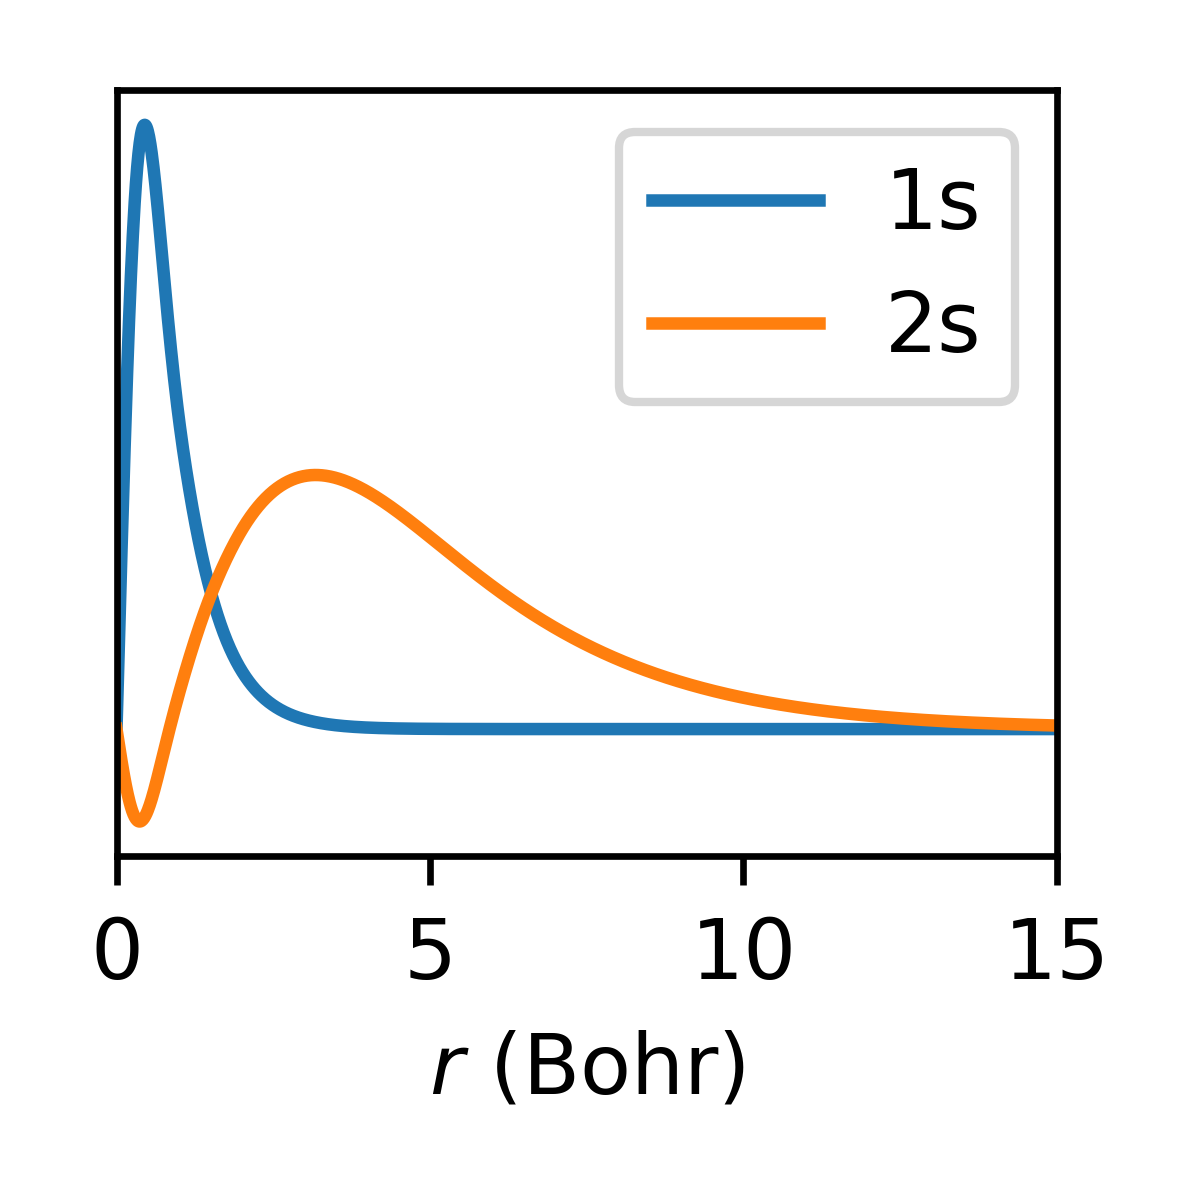
\includegraphics[width=0.8\columnwidth]{figures/plot_paos/old_projs.png}}
               \only<3>{\includegraphics[height=0.6\paperheight]{figures/proj_disentanglement_fig1a.png}}
               \only<4>{\includegraphics[width=\columnwidth]{figures/target_manifolds_fig1b.png}}
            \end{center}
         \end{overlayarea}
      \end{column}
   \end{columns}
   % \begin{figure}[t]
   %    \begin{subfigure}{0.2\textwidth}
   %       \onslide<2->{
   %       \includegraphics[height=1.5\columnwidth]{figures/proj_disentanglement_fig1b.png}
   %       \vspace{-0.01\paperheight}
   %       }
   %    \end{subfigure}
   %    \begin{subfigure}{0.2\textwidth}
   %    \onslide<3->{
   %       \includegraphics[height=1.5\columnwidth]{figures/proj_disentanglement_fig1a.png}
   %    }
   % \end{subfigure}
   %    \hspace{0.025\textwidth}
   %    % \begin{subfigure}{0.225\textwidth}
   %    %    \onslide<3->{
   %    %    \includegraphics[height=1.5\columnwidth]{figures/proj_disentanglement_fig1d.png}
   %    %    }
   %    % \end{subfigure}
   %    \begin{subfigure}{0.2\textwidth}
   %       \onslide<4->{
   %       \includegraphics[height=1.5\columnwidth]{figures/proj_disentanglement_fig1f.png}
   %       }
   %    \end{subfigure}
   % \end{figure}

   \blfootcite{Agapito2013}
   \blfootcite{Qiao2023,Qiao2023a}

\end{frame}

\begin{frame}{Automated Wannierisation}
   \vspace{-2ex}
   \begin{columns}
      \begin{column}{0.5\textwidth}
         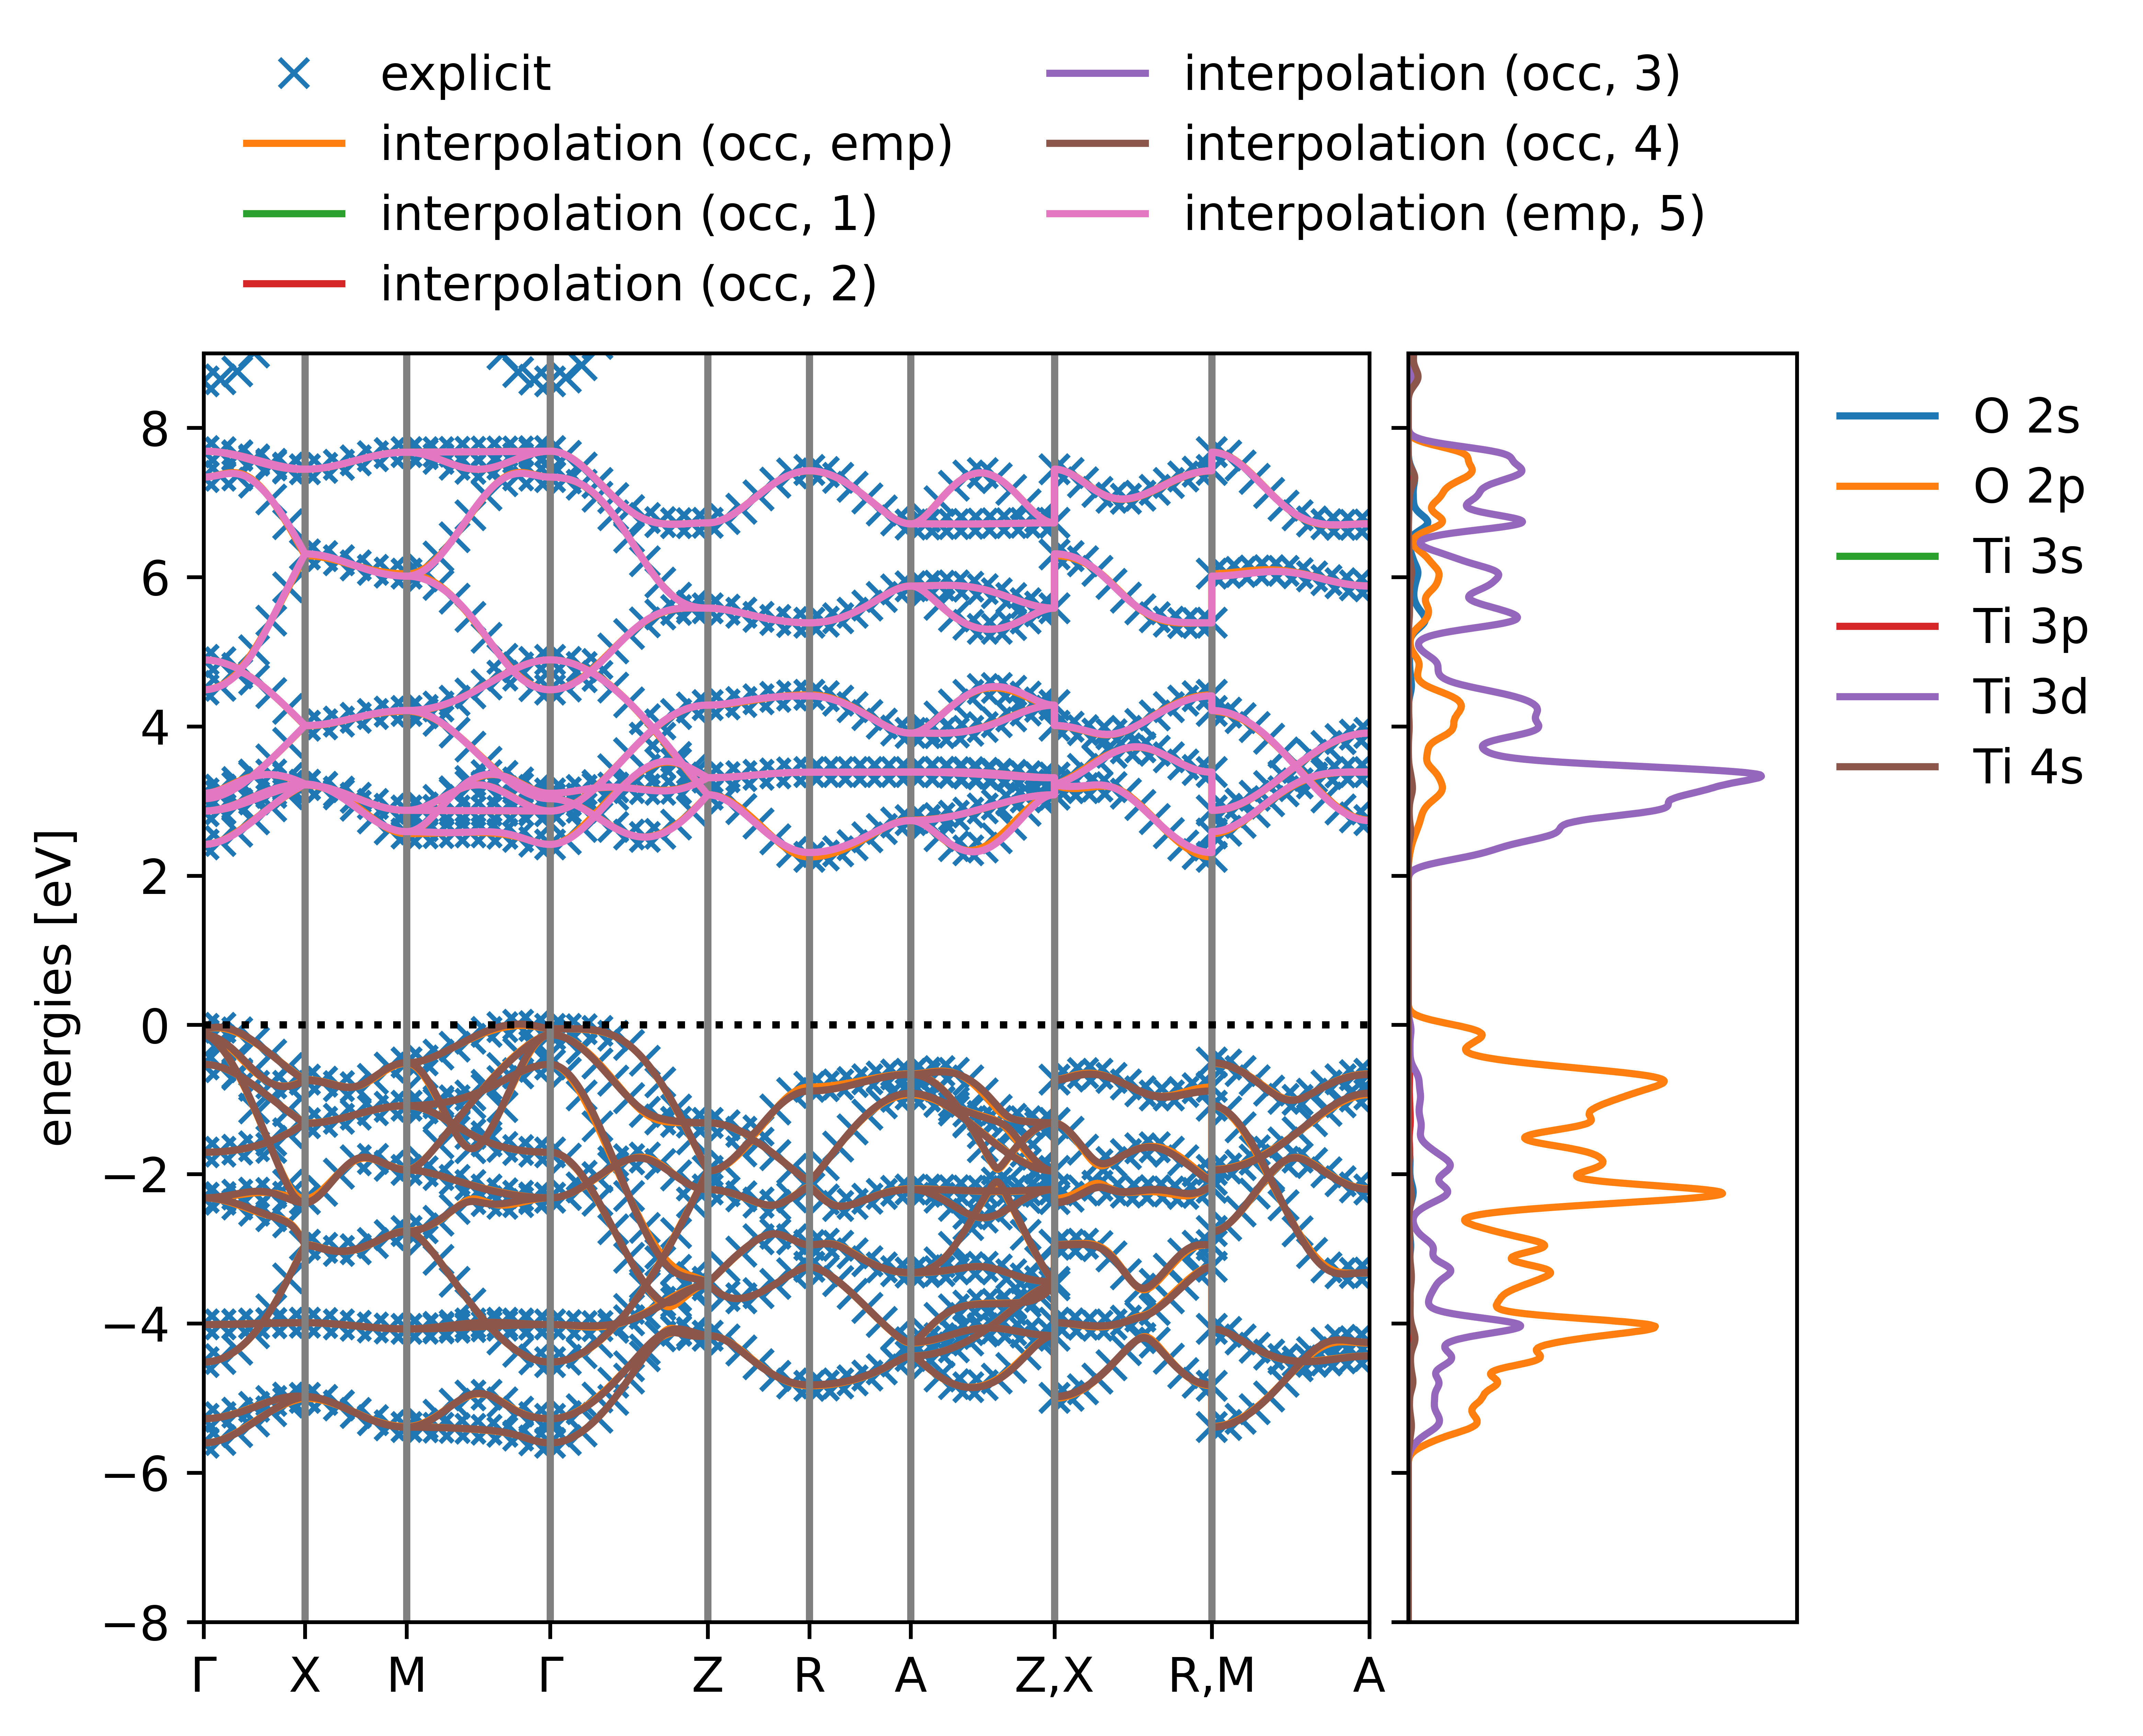
\includegraphics[width=\columnwidth]{figures/TiO2_wannierize_bandstructure.png}
      \end{column}
      \begin{column}{0.5\textwidth}
         \onslide<2->{
            \inputminted[fontsize=\tiny]{json}{scripts/TiO2.json}
         }
      \end{column}
      % \hbox{
      %    \raisebox{0.15\textwidth}{\huge $\rightarrow$}
      % }
   \end{columns}
\end{frame}

\begin{frame}{Automated Wannierisation}

   A drawback: the number of Wannier functions is determined by the number of PAOs in the pseudopotentials\onslide<2->{... which can be a problem e.g. LiF}

   \begin{columns}
      \begin{column}{0.5\textwidth}
         \onslide<3->{

            \begin{center}
               \footnotesize
               \begin{tabular}[h]{ccc}
                  element & configuration                                                                                             & {PAOs}                                                              \\
                  \hline
                  Li      & 1s\textsuperscript{2} 2s\textsuperscript{1}                                                               & {1s, 2s}                                                            \\
                  {F}     & {\textcolor{seaborn_bg_grey_darker}{[1s\textsuperscript{2}]} 2s\textsuperscript{2} 2p\textsuperscript{5}} & {2s, 2p\textsubscript{x}, 2p\textsubscript{y}, 2p\textsubscript{z}} \\
               \end{tabular}
            \end{center}
         }
         \vspace{1ex}
         \onslide<5->{If we want a better representation of the conduction bands, we're gonna need \sout{a bigger boat} more PAOs...}
      \end{column}
      \begin{column}{0.5\textwidth}
         \vspace{1ex}
         \onslide<4->{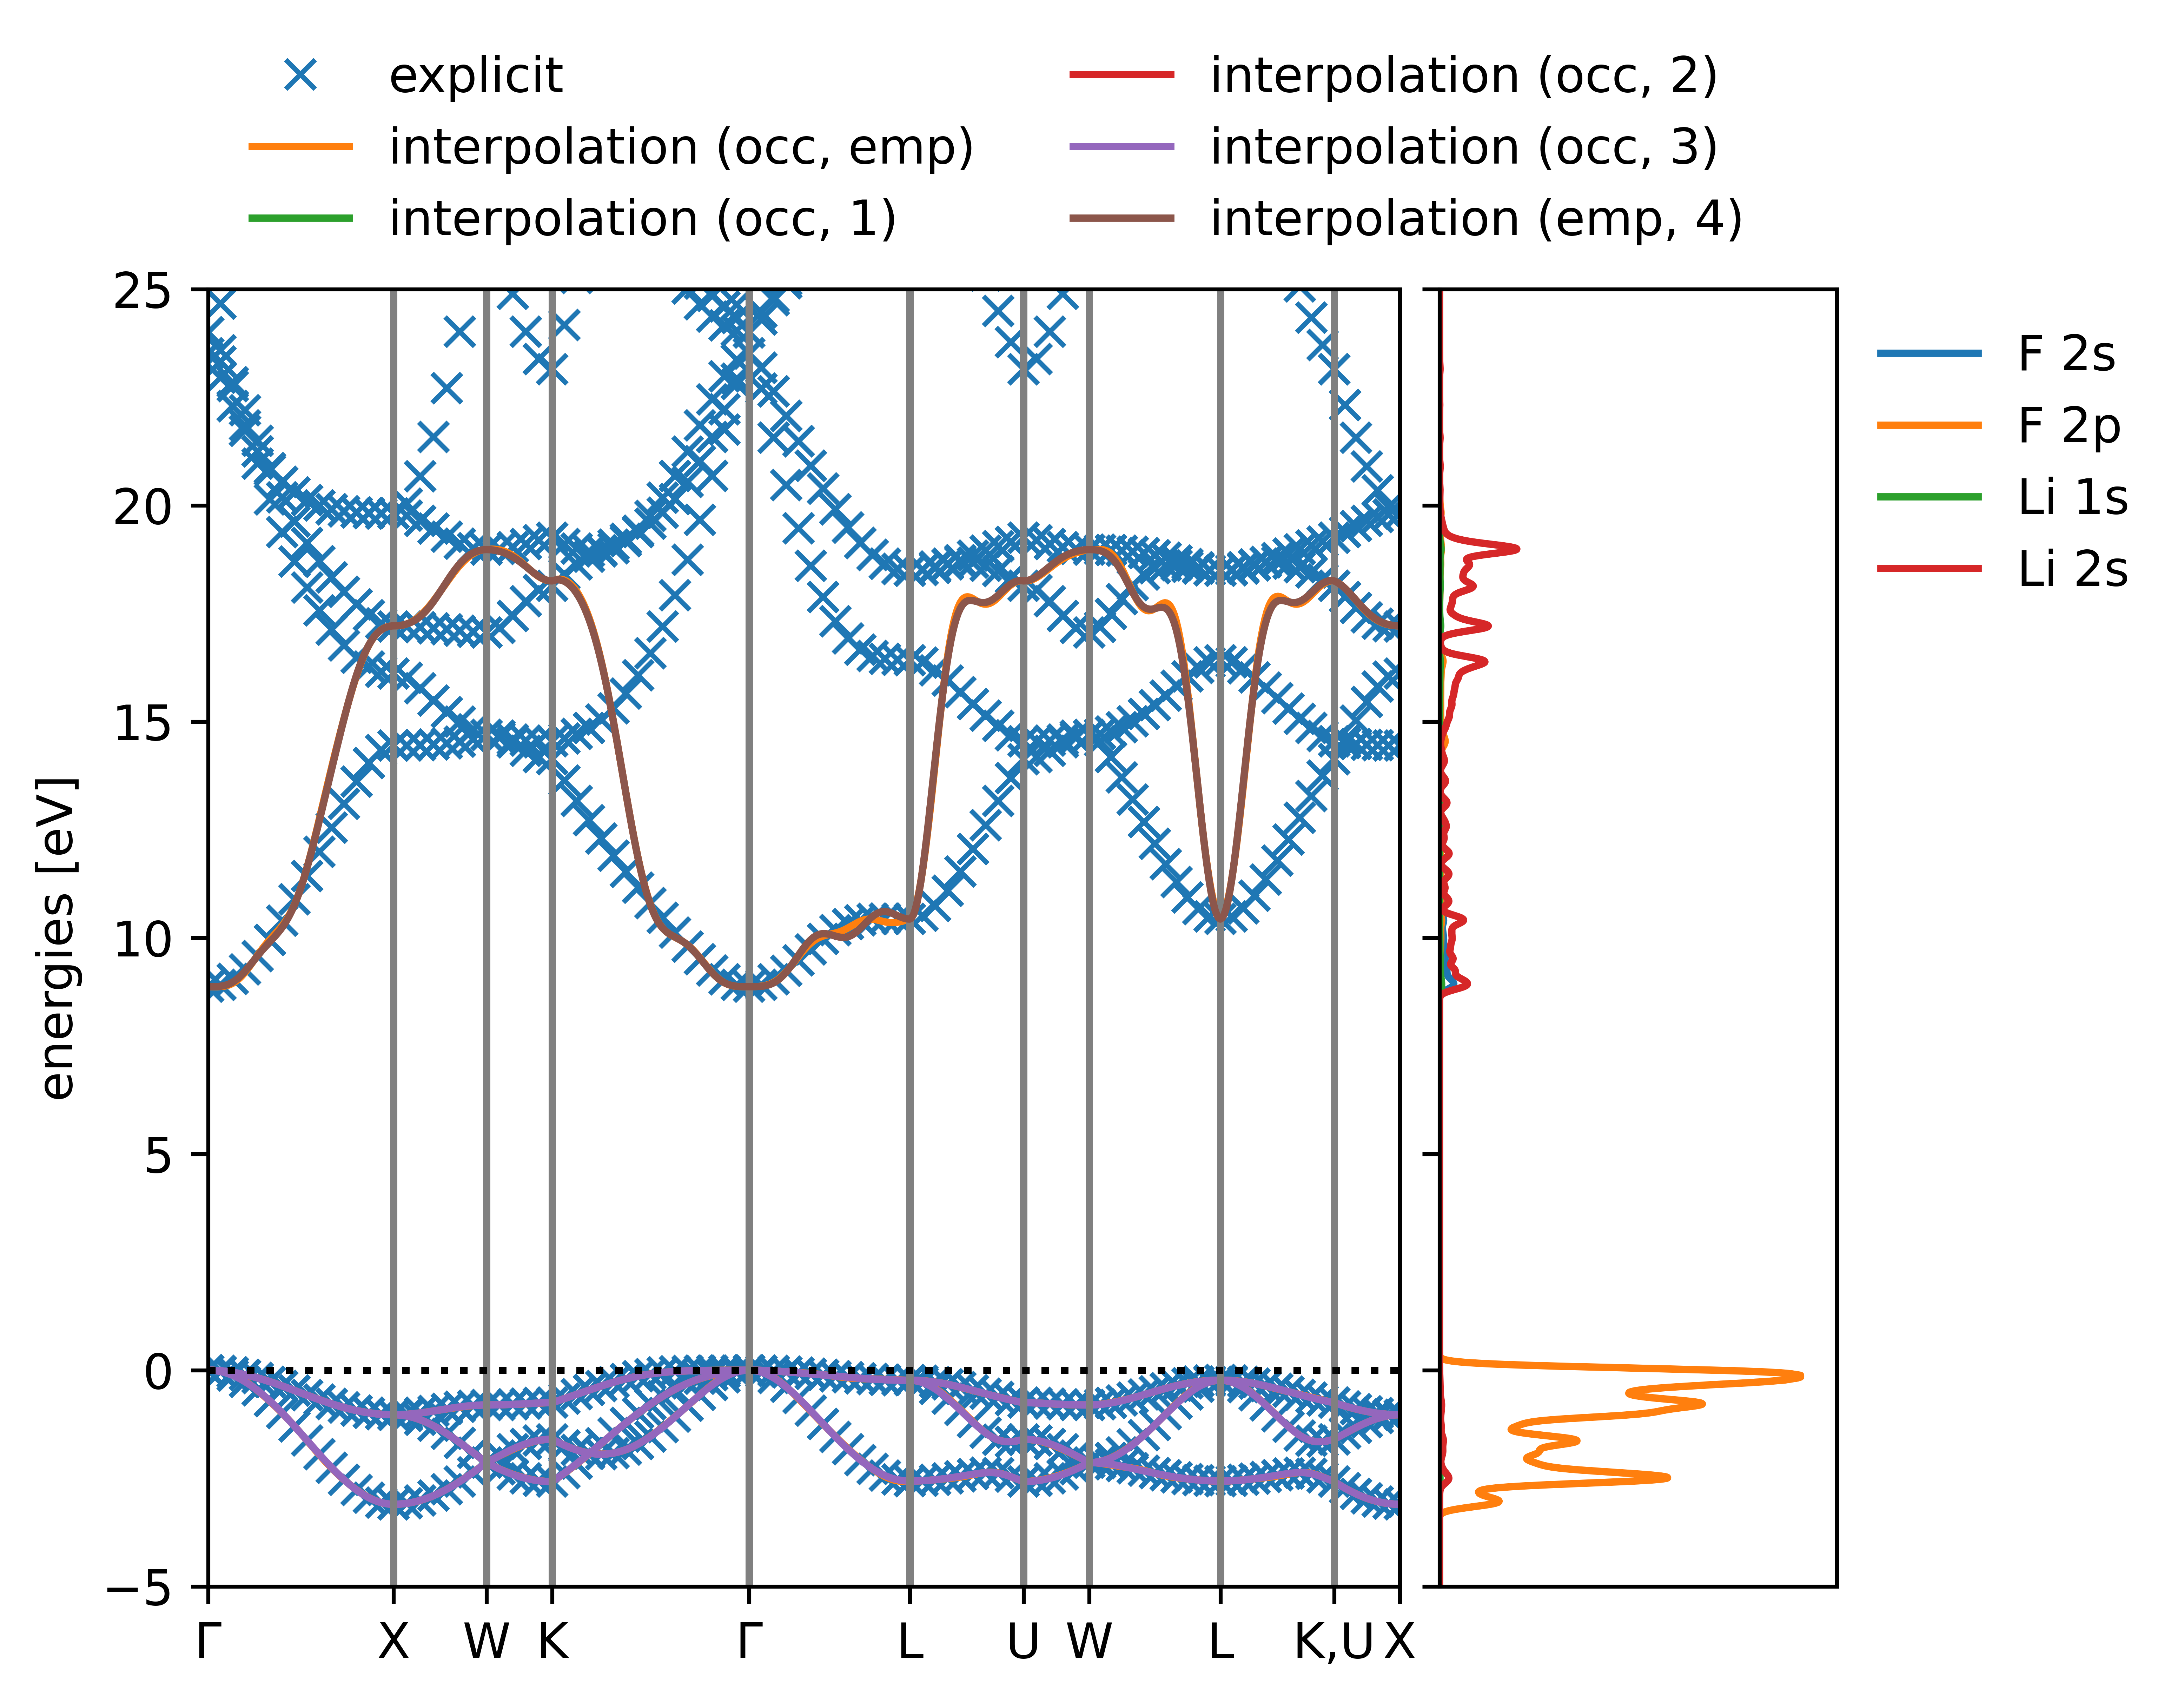
\includegraphics[width=\textwidth]{figures/LiF_bandstructures/default.png}}

      \end{column}

   \end{columns}
\end{frame}

% \begin{frame}{Automating Wannierization}
% 
%    Pseudoatomic orbitals play a dual purpose
%    \begin{itemize}
%       \item we use them to calculate projectability \onslide<2->{$\rightarrow$ we rely on the PAOs having high overlap with the atomic-like bands}
%       \item they serve as our initial guesses for the Wannier functions \onslide<3->{$\rightarrow$ the number of Wannier functions is limited to the number of pseudoatomic orbitals}
%    \end{itemize}
% 
%    \onslide<4->{e.g. LiF}
% 
%    \onslide<5->{
% 
%       \begin{center}
%          \begin{tabular}[h]{cccc}
%             element         & electronic configuration                                                                                              & \onslide<6->{PAOs}                                                              & \onslide<7->{number of PAOs} \\
%             \hline
%             Li              & 1s\textsuperscript{2} 2s\textsuperscript{1}                                                                           & \onslide<6->{1s, 2s}                                                            & \onslide<7->{2}              \\
%             \onslide<8->{F} & \onslide<8->{\textcolor{seaborn_bg_grey_darker}{[1s\textsuperscript{2}]} 2s\textsuperscript{2} 2p\textsuperscript{5}} & \onslide<9->{2s, 2p\textsubscript{x}, 2p\textsubscript{y}, 2p\textsubscript{z}} & \onslide<9->{4}
%          \end{tabular}
%       \end{center}
%    }
% 
%    \vspace{1ex}
%    \onslide<10->{6 Wannier functions for a system with 10 electrons} \onslide<11->{= 5 occupied bands + only 1 unoccupied band!}
% 
%    \vspace{1ex}
%    \onslide<12->{If we want more Wannier functions, we're gonna need \sout{a bigger boat} more PAOs...}
% 
% \end{frame}

\begin{frame}{Automated Wannierization}
   \begin{tabular}{p{0.3\textwidth} p{0.65\textwidth}}
   \multicolumn{1}{c}{\textbf{old}} & \multicolumn{1}{c}{\onslide<2->{\textbf{new}}} \\
   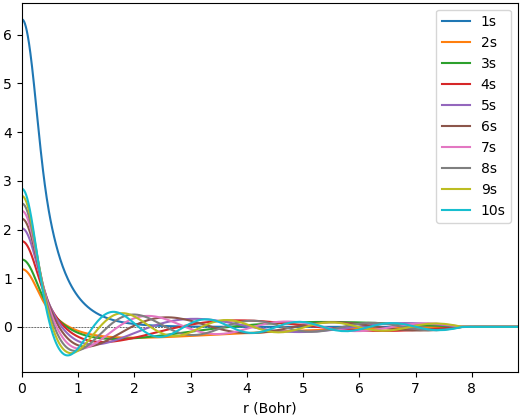
\includegraphics[width=0.28\textwidth]{figures/Li8.0.pao_10_0_0_0_cropped.png}
   &
   \leavevmode\onslide<2->{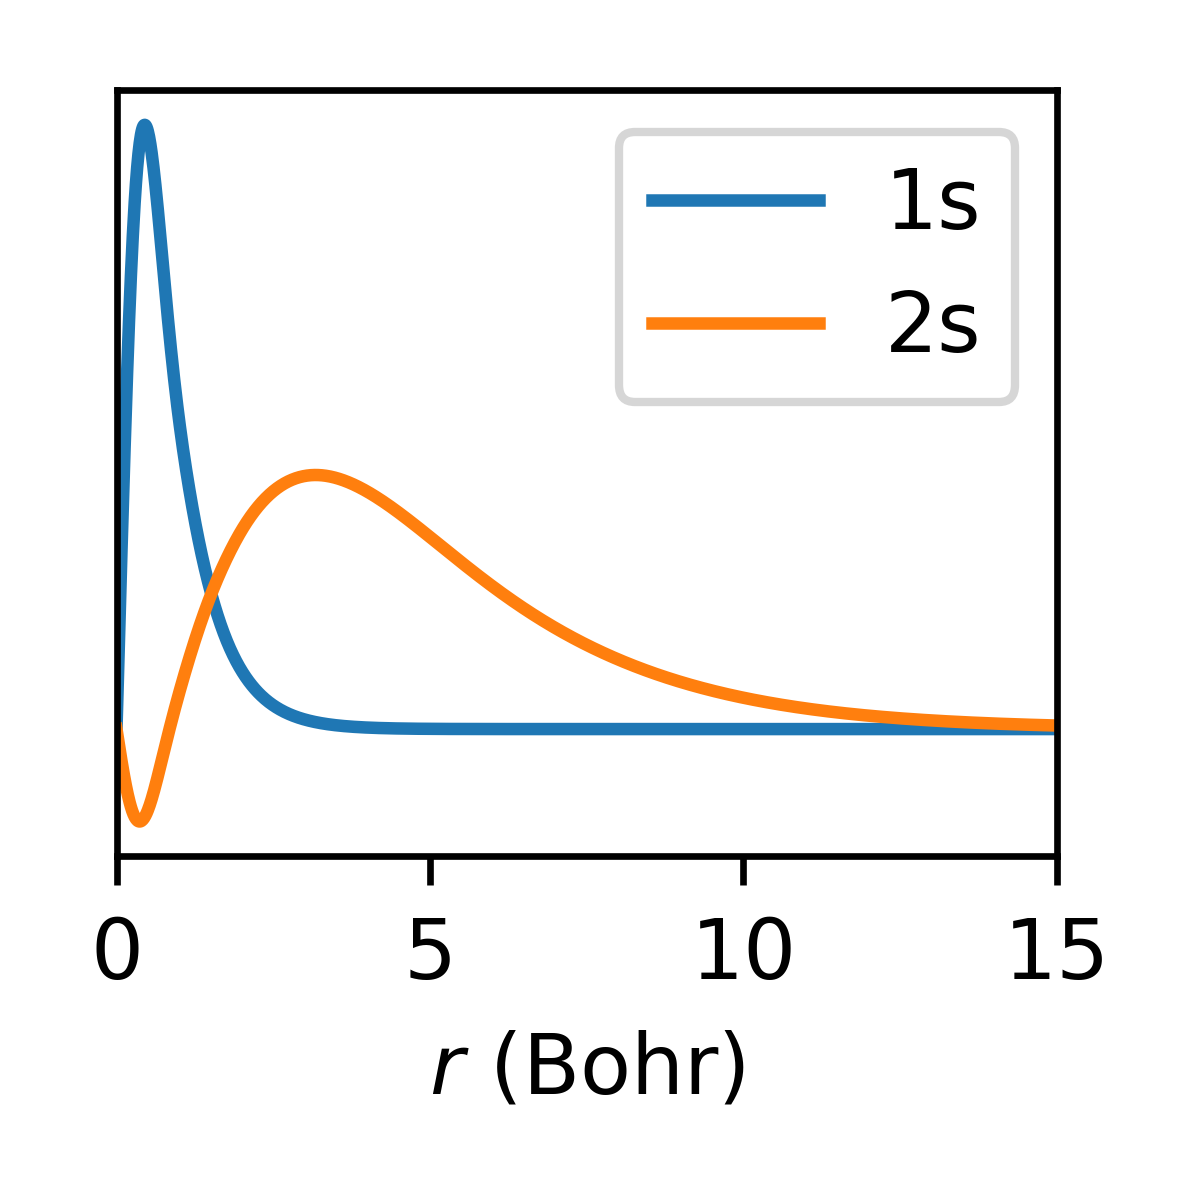
\includegraphics[width=0.26\textwidth]{figures/plot_paos/old_projs.png} %
   \raisebox{0.125\textwidth}{\huge $\rightarrow$} %
   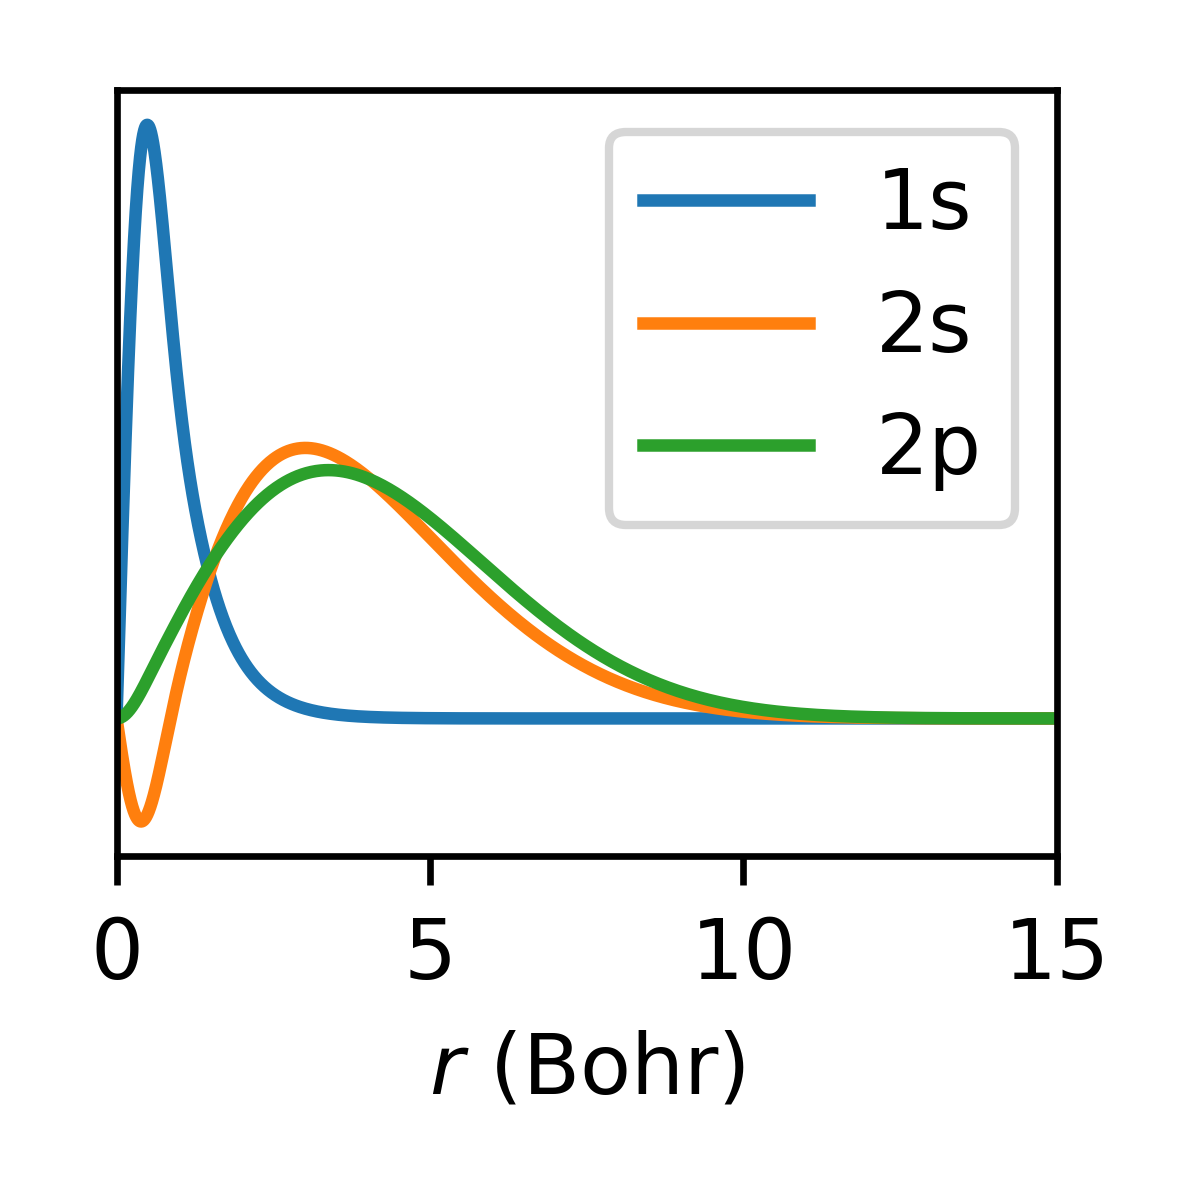
\includegraphics[width=0.26\textwidth]{figures/plot_paos/new_projs.png}} \\
   use the PAOs provided by OpenMX &
   \onslide<2->{for the pseudopotential in question, resolve the radial Schrödinger equation for the next subshell}
   \end{tabular}

\end{frame}

\begin{frame}{}
   \begin{center}
      \Huge \bf Pseudopotential generation
   \end{center}
\end{frame}

\begin{frame}{Pseudopotential generation}
   \textbf{Solving the KS equations for a radial scalar-relativistic potential}

   \onslide<2->{%
   Solved on a logarithmic grid
   \begin{equation*}
      r_i = r_0 e^{i \Delta x}
   \end{equation*}
   }

   \onslide<3->{%
   Start with a trial potential $V[n](r)$ and eigenvalue $\varepsilon$. Then the radial wavefunction $R_{nl}$ satisfies
   \begin{align*}
      \frac{1}{r^2} \frac{d^2 R_{n l}(x)}{d x^2}= & \frac{1}{r^2} \frac{d R_{n l}(x)}{d x}+\left(\frac{l(l+1)}{r^2}+M(r)(V(r)-\varepsilon)\right) R_{n l}(r)                                    \\
                                                  & -\frac{\alpha^2}{4 M(r)} \frac{d V(r)}{d r}\left(\frac{1}{r} \frac{d R_{n l}(x)}{d x} - \frac{R_{n l}(r)}{r}\right) .
   \end{align*}
   where $M(r) = 1-\frac{\alpha^2}{4}(V(r)-\varepsilon)$
   }

\end{frame}
\begin{frame}{Solving scalar-relativisitic radial KS}

   Extrapolate outwards from the known small-$r$ behaviour
   \begin{align*}
      R_{nl}(r) \sim r^\gamma; \qquad \gamma=\frac{l \sqrt{l^2-\alpha^2 Z^2}+(l+1) \sqrt{(l+1)^2-\alpha^2 Z^2}}{2 l+1}
   \end{align*}

   \onslide<2->{%
   Extrapolate inwards from the known large-$r$ behaviour
   \begin{align*}
      R_{n l}(r) \sim e^{-k(r) r}, \quad k(r)=\sqrt{\frac{l(l+1)}{r^2}+(V(r)-\epsilon)}
   \end{align*}
   }

   \begin{itemize}[<+(3)->]
      \item if the wavefunction has too many/few nodes, $\varepsilon$ is too high/low
      \item if the wavefunction has a discontinuity where the outward and inward solutions intercept, we can estimate how much $\varepsilon$ needs to change via perturbation theory
      \item if the wavefunction does not have a discontinuity, we have found a solution! Now cycle for self-consistency over $V[n[(r)$
   \end{itemize}

\end{frame}

\begin{frame}{Pseudopotential generation}
   Use this procedure to generate extra PAOs for the Wannierisation

   \onslide<2->{
      \vspace{1ex}
      Problem: extra bound states may not exist
   }

   \onslide<3->{
      \vspace{1ex}
      Solution: add a confining potential
   }

   \onslide<4->{
      \vspace{1ex}
      Problem: how to choose the confining potential parameters?
   }

   \onslide<5->{
      Solution: optimise these criteria across typical structures:

      \begin{center}
         \footnotesize
      \begin{tabular}{ccccc}
         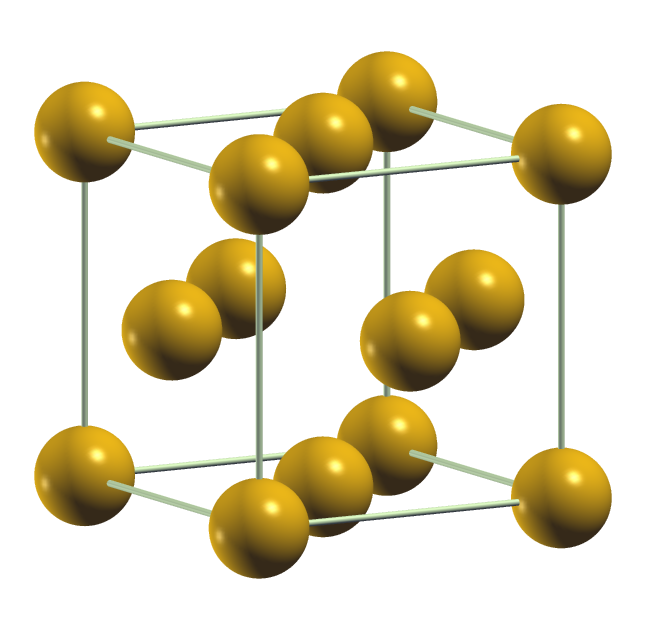
\includegraphics[width=0.125\textwidth]{figures/sssp_structures/P-FCC-conv.png} &
         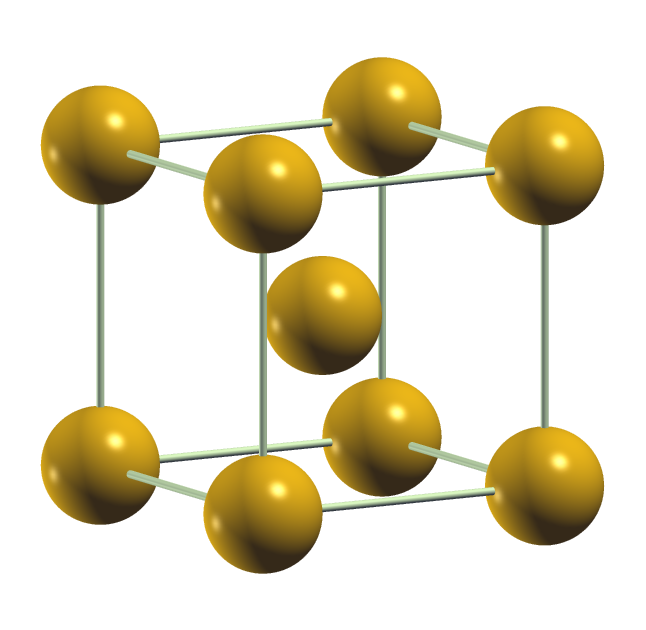
\includegraphics[width=0.125\textwidth]{figures/sssp_structures/P-BCC-conv.png} &
         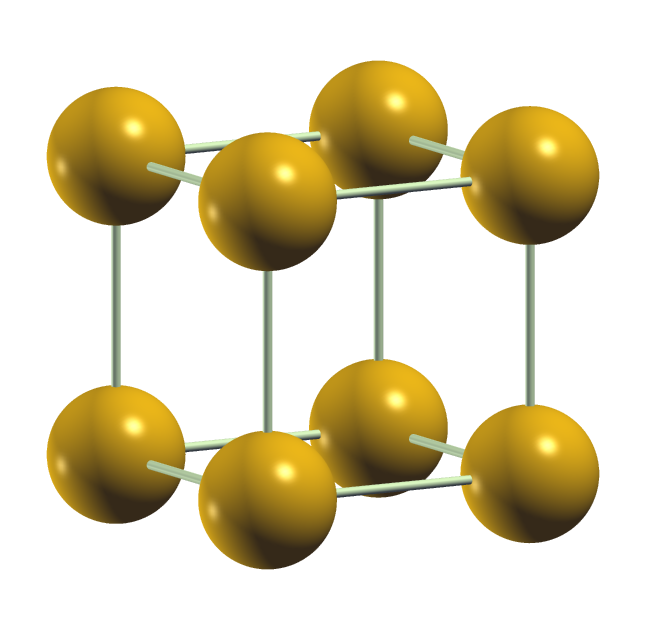
\includegraphics[width=0.125\textwidth]{figures/sssp_structures/P-SC-conv.png} &
         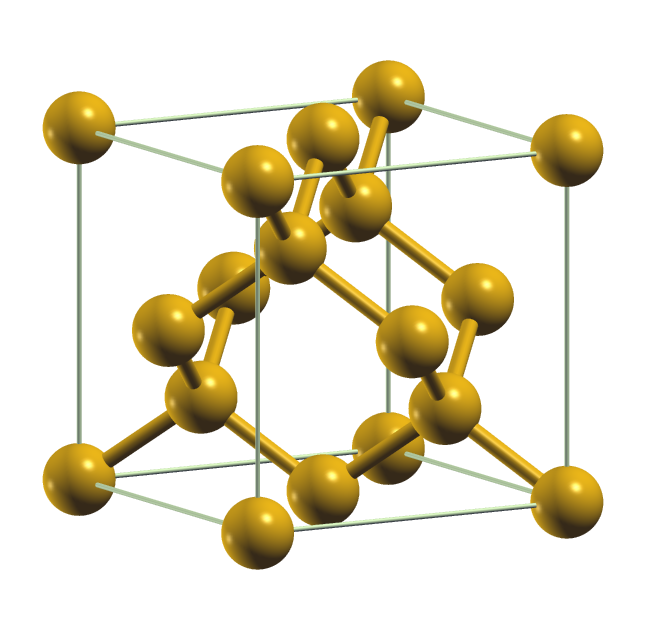
\includegraphics[width=0.125\textwidth]{figures/sssp_structures/P-Diamond-conv.png} &
         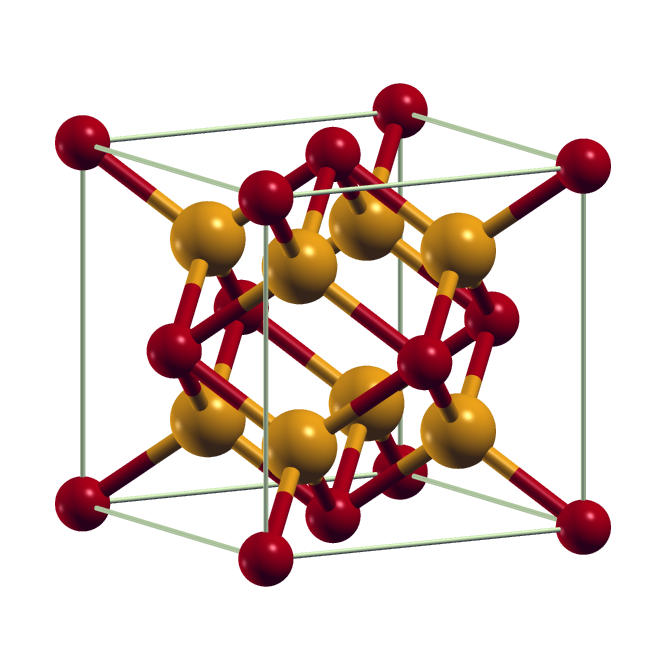
\includegraphics[width=0.125\textwidth]{figures/sssp_structures/P-X2O-conv_cell.png} \\
         FCC & BCC & SC & Diamond & X\textsubscript{2}O \\
         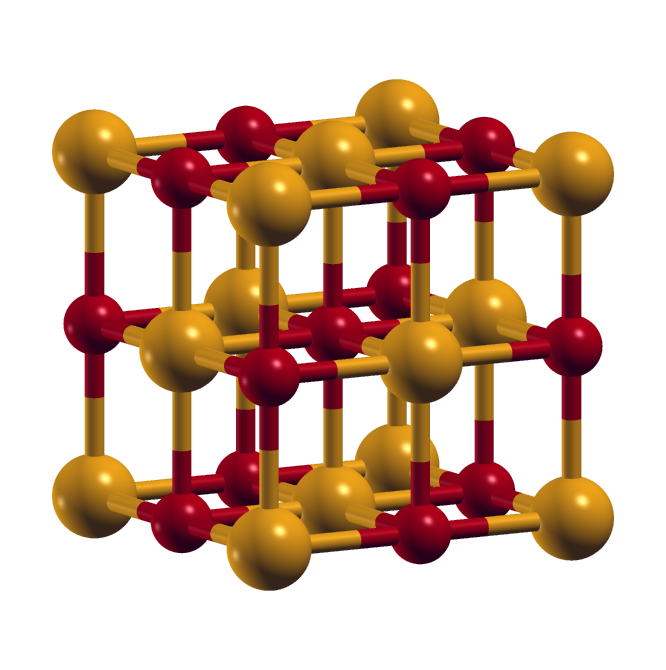
\includegraphics[width=0.125\textwidth]{figures/sssp_structures/P-XO-conv_cell.png} &
         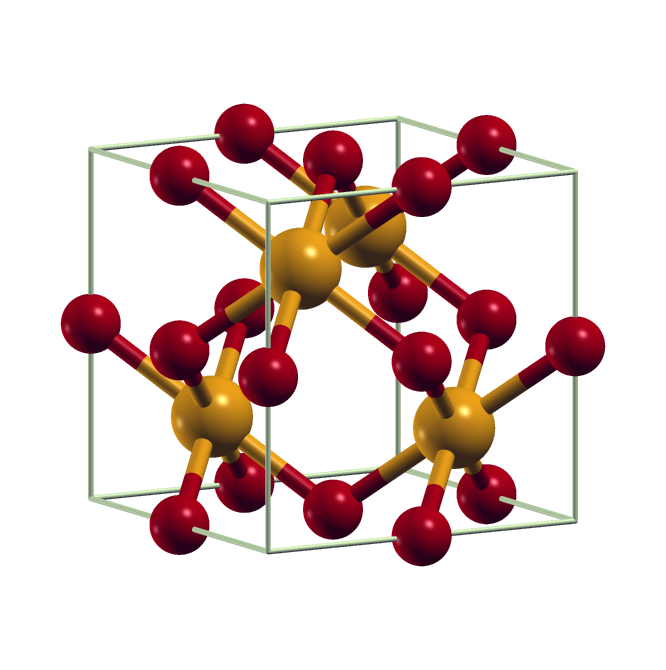
\includegraphics[width=0.125\textwidth]{figures/sssp_structures/P-X2O3-conv_cell.png} &
         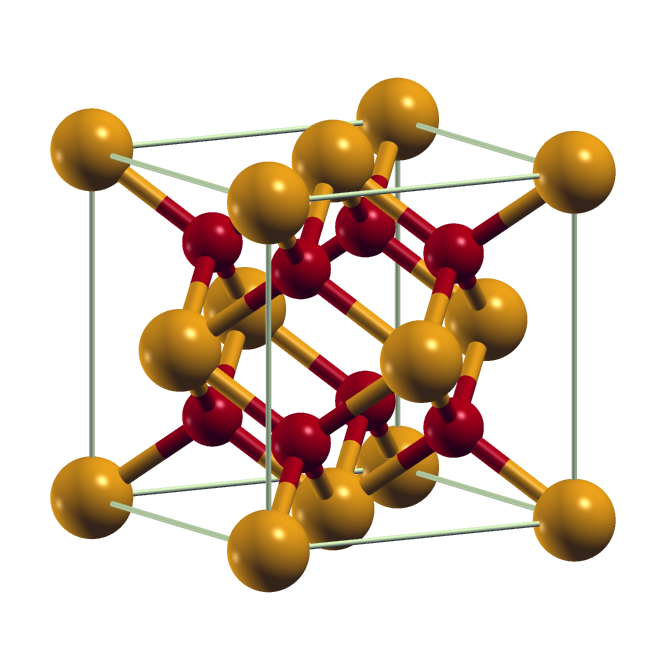
\includegraphics[width=0.125\textwidth]{figures/sssp_structures/P-XO2-conv_cell.png} &
         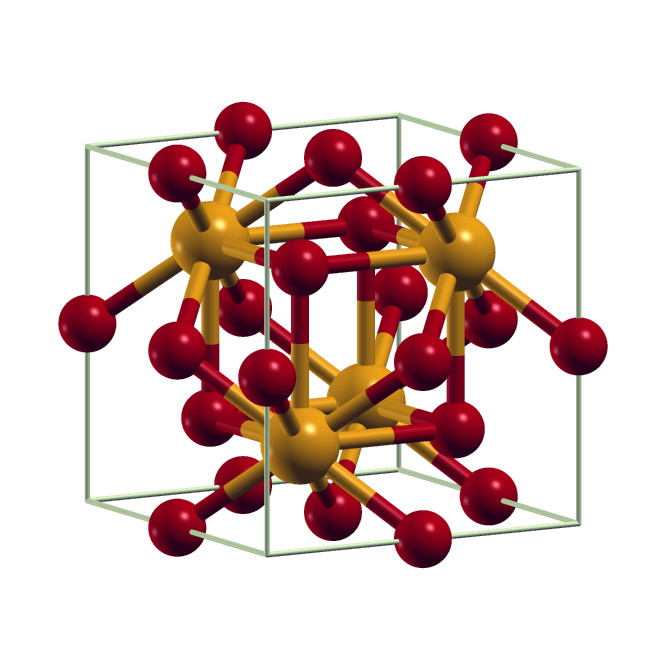
\includegraphics[width=0.125\textwidth]{figures/sssp_structures/P-X2O5-conv_cell.png} &
         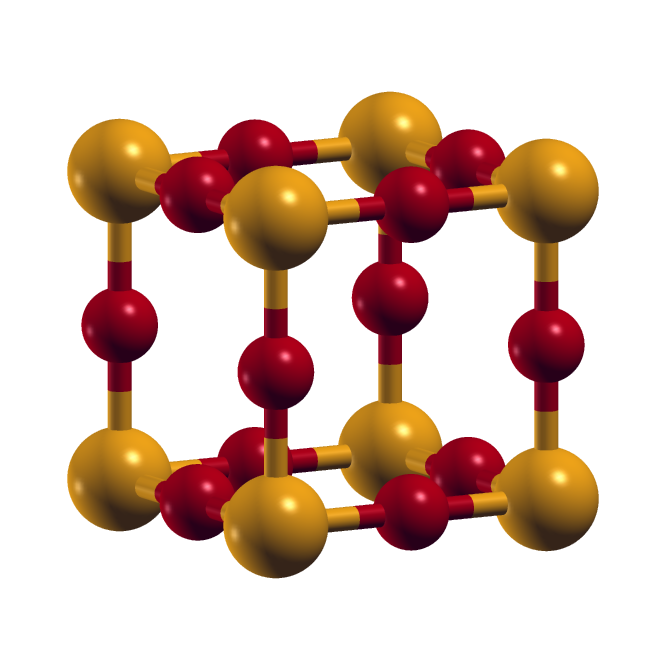
\includegraphics[width=0.125\textwidth]{figures/sssp_structures/P-XO3-conv_cell.png} \\
         XO & X\textsubscript{2}O\textsubscript{3} & XO\textsubscript{2} & X\textsubscript{2}O\textsubscript{5} & XO\textsubscript{3}
      \end{tabular}
   \end{center}
   }
\end{frame}

\begin{frame}{Pseudopotential generation}

   The projectability is
   \begin{equation*}
      p_{m\mathbf{k}} = \sum_n |\langle \varphi_n \mid \psi_{m\mathbf{k}}\rangle |^2
   \end{equation*}

   \onslide<2->{
   \vspace{1ex}
   We want a set of projectors such that\dots
   \begin{itemize}
      \item they should have a large overlap with some Kohn-Sham states and a small overlap with all the others% i.e. $p_{m\mathbf{k}}$ should be close to 0 or 1 for all $m$ and $\mathbf{k}$
      \item they should lie within the span of the Kohn-Sham states% i.e. $\sum_{m\mathbf{k}} p_{m\mathbf{k}}$ should be as large as possible
   \end{itemize}
   }

   \onslide<3->{
   \vspace{1ex}
   We can meet these criteria if we maximise the functional
   \begin{equation*}
      F[\{\varphi_n\}] = \frac{1}{N_\mathbf{k} N_w} \sum_{\mathbf{k}} \sum_{m \in \mathcal{S}_\mathbf{k}} p_{m\mathbf{k}}
   \end{equation*}

   where $\mathcal{S}_\mathbf{k}$ corresponds to the $N_w$-largest values of $p_{m\mathbf{k}}$.
   }

   \onslide<4->{
   \vspace{1ex}
   Maximise via \emph{Bayesian optimisation}
   }
\end{frame}


\begin{frame}{Pseudopotential generation}
   \begin{center}
   \only<1>{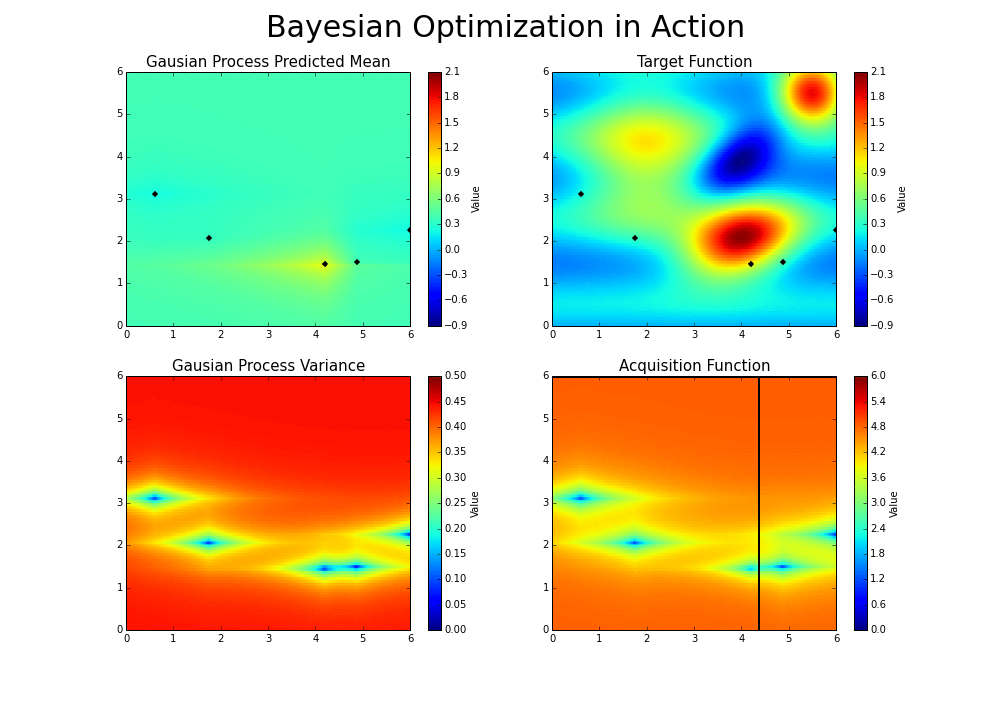
\includegraphics[height=0.7\textheight]{figures/bayesian_optimisation/frame_00_delay-0.5s.png}}%
   \only<2>{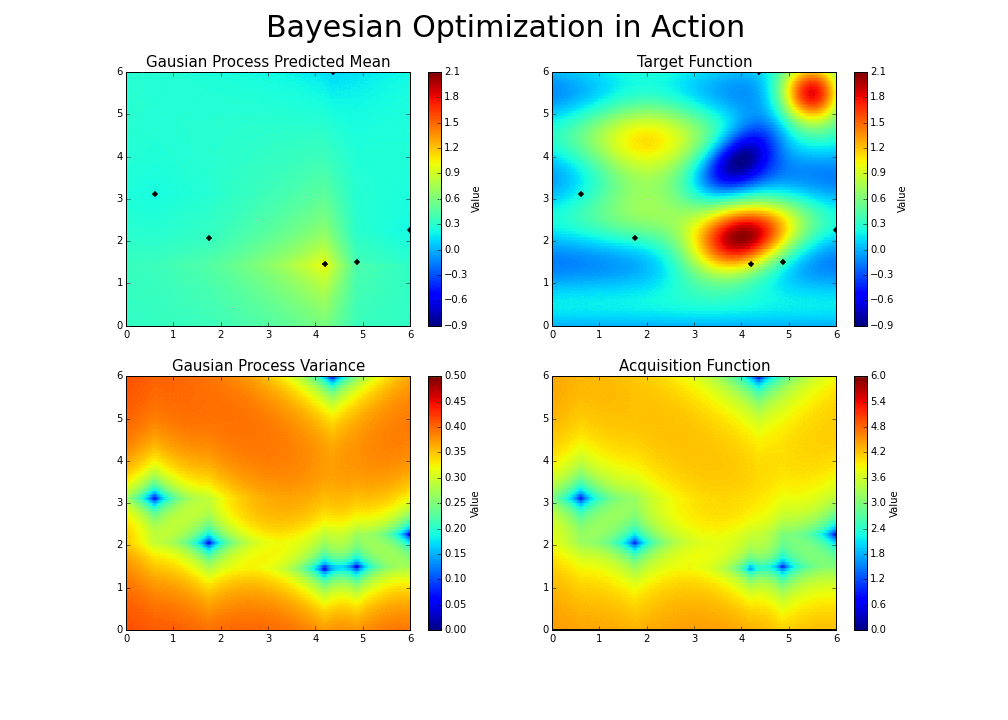
\includegraphics[height=0.7\textheight]{figures/bayesian_optimisation/frame_01_delay-0.5s.png}}%
   \only<3>{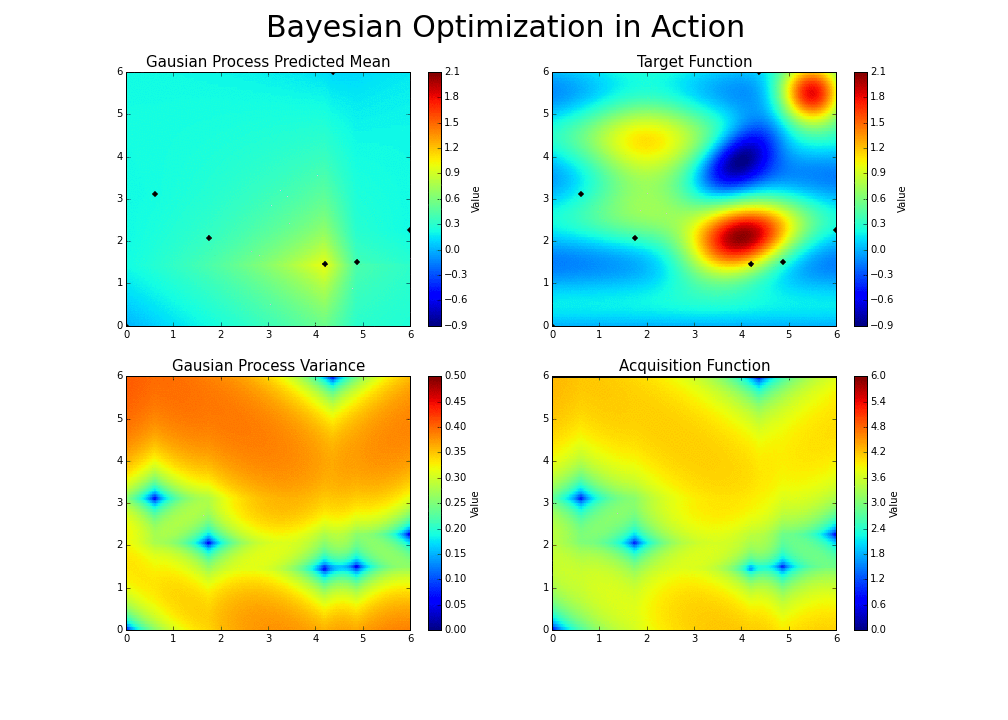
\includegraphics[height=0.7\textheight]{figures/bayesian_optimisation/frame_02_delay-0.5s.png}}%
   \only<4>{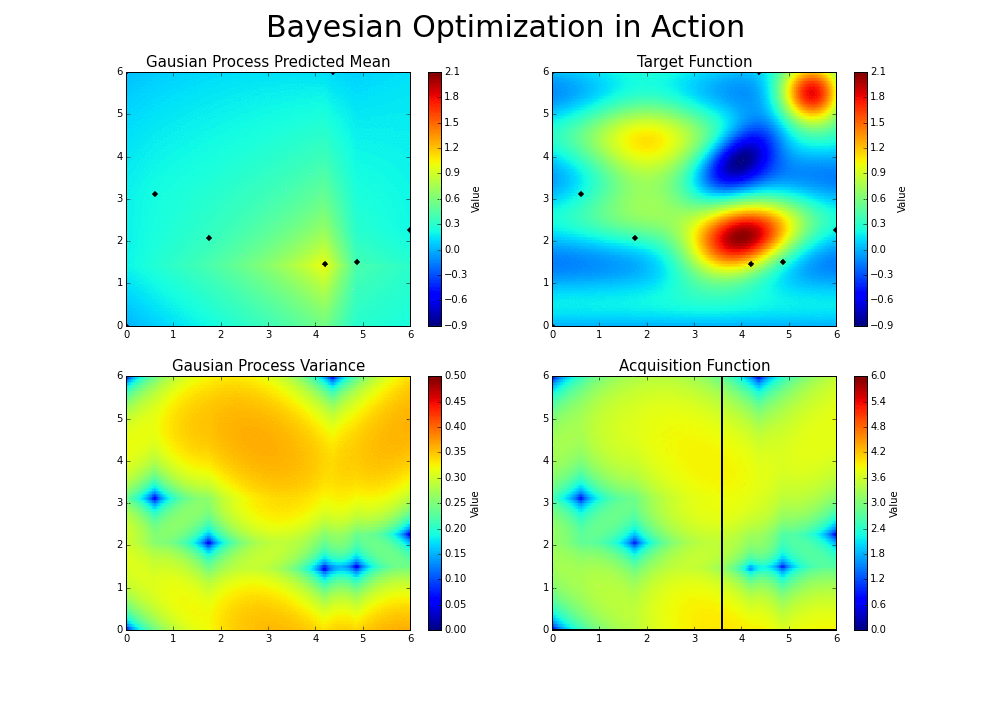
\includegraphics[height=0.7\textheight]{figures/bayesian_optimisation/frame_03_delay-0.5s.png}}%
   \only<5>{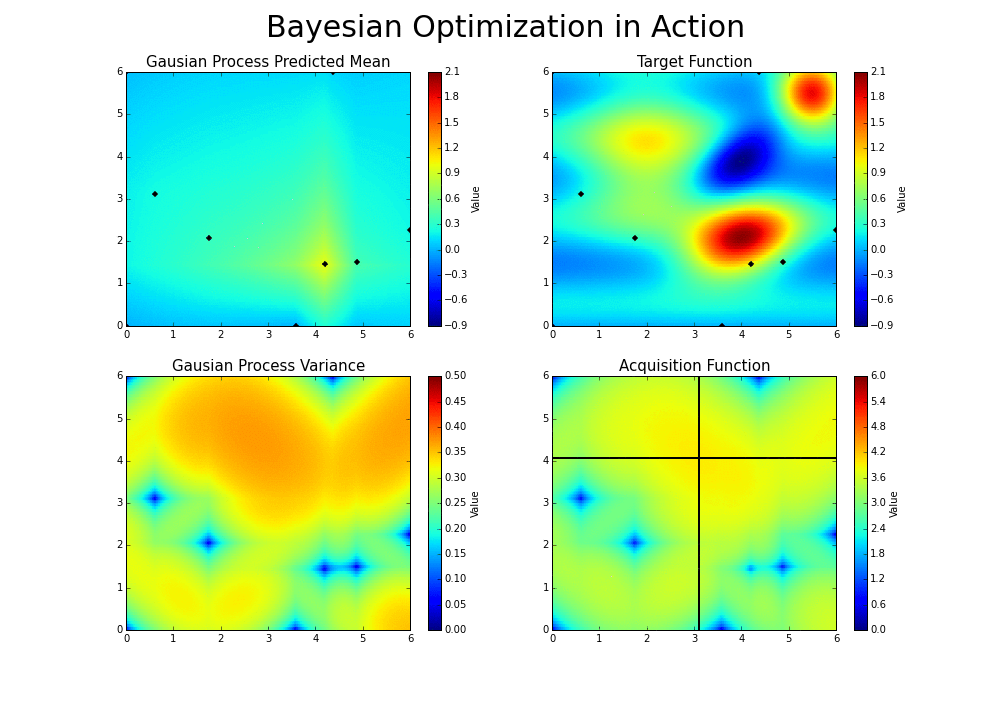
\includegraphics[height=0.7\textheight]{figures/bayesian_optimisation/frame_04_delay-0.5s.png}}%
   \only<6>{\includegraphics[height=0.7\textheight]{figures/bayesian_optimisation/frame_05_delay-0.5s.png}}%
   \only<7>{\includegraphics[height=0.7\textheight]{figures/bayesian_optimisation/frame_06_delay-0.5s.png}}%
   \only<8>{\includegraphics[height=0.7\textheight]{figures/bayesian_optimisation/frame_07_delay-0.5s.png}}%
   \only<9>{\includegraphics[height=0.7\textheight]{figures/bayesian_optimisation/frame_08_delay-0.5s.png}}%
   \only<10>{\includegraphics[height=0.7\textheight]{figures/bayesian_optimisation/frame_09_delay-0.5s.png}}%
   \only<11>{\includegraphics[height=0.7\textheight]{figures/bayesian_optimisation/frame_10_delay-0.5s.png}}%
   \only<12>{\includegraphics[height=0.7\textheight]{figures/bayesian_optimisation/frame_11_delay-0.5s.png}}%
   \only<13>{\includegraphics[height=0.7\textheight]{figures/bayesian_optimisation/frame_12_delay-0.5s.png}}%
   \only<14>{\includegraphics[height=0.7\textheight]{figures/bayesian_optimisation/frame_13_delay-0.5s.png}}%
   \only<15>{\includegraphics[height=0.7\textheight]{figures/bayesian_optimisation/frame_14_delay-0.5s.png}}%
   \only<16>{\includegraphics[height=0.7\textheight]{figures/bayesian_optimisation/frame_15_delay-0.5s.png}}%
   \only<17>{\includegraphics[height=0.7\textheight]{figures/bayesian_optimisation/frame_16_delay-0.5s.png}}%
   \only<18>{\includegraphics[height=0.7\textheight]{figures/bayesian_optimisation/frame_17_delay-0.5s.png}}%
   \only<19>{\includegraphics[height=0.7\textheight]{figures/bayesian_optimisation/frame_18_delay-0.5s.png}}%
   \only<20>{\includegraphics[height=0.7\textheight]{figures/bayesian_optimisation/frame_19_delay-0.5s.png}}%
   \only<21>{\includegraphics[height=0.7\textheight]{figures/bayesian_optimisation/frame_20_delay-0.5s.png}}%
   \only<22>{\includegraphics[height=0.7\textheight]{figures/bayesian_optimisation/frame_21_delay-0.5s.png}}%
   \only<23>{\includegraphics[height=0.7\textheight]{figures/bayesian_optimisation/frame_22_delay-0.5s.png}}%
   \only<24>{\includegraphics[height=0.7\textheight]{figures/bayesian_optimisation/frame_23_delay-0.5s.png}}%
   \only<25>{\includegraphics[height=0.7\textheight]{figures/bayesian_optimisation/frame_24_delay-0.5s.png}}%
   \only<26>{\includegraphics[height=0.7\textheight]{figures/bayesian_optimisation/frame_25_delay-0.5s.png}}%
   \only<27>{\includegraphics[height=0.7\textheight]{figures/bayesian_optimisation/frame_26_delay-0.5s.png}}%
   \only<28>{\includegraphics[height=0.7\textheight]{figures/bayesian_optimisation/frame_27_delay-0.5s.png}}%
   \only<29>{\includegraphics[height=0.7\textheight]{figures/bayesian_optimisation/frame_28_delay-0.5s.png}}%
   \only<30>{\includegraphics[height=0.7\textheight]{figures/bayesian_optimisation/frame_29_delay-0.5s.png}}%
   \only<31>{\includegraphics[height=0.7\textheight]{figures/bayesian_optimisation/frame_30_delay-0.5s.png}}%
   \only<32>{\includegraphics[height=0.7\textheight]{figures/bayesian_optimisation/frame_31_delay-0.5s.png}}%
   \only<33>{\includegraphics[height=0.7\textheight]{figures/bayesian_optimisation/frame_32_delay-0.5s.png}}%
   \only<34>{\includegraphics[height=0.7\textheight]{figures/bayesian_optimisation/frame_33_delay-0.5s.png}}%
   \only<35>{\includegraphics[height=0.7\textheight]{figures/bayesian_optimisation/frame_34_delay-0.5s.png}}%
   \only<36>{\includegraphics[height=0.7\textheight]{figures/bayesian_optimisation/frame_35_delay-0.5s.png}}%
   \only<37>{\includegraphics[height=0.7\textheight]{figures/bayesian_optimisation/frame_36_delay-0.5s.png}}%
   \only<38>{\includegraphics[height=0.7\textheight]{figures/bayesian_optimisation/frame_37_delay-0.5s.png}}%
   \only<39>{\includegraphics[height=0.7\textheight]{figures/bayesian_optimisation/frame_38_delay-0.5s.png}}%
   \only<40>{\includegraphics[height=0.7\textheight]{figures/bayesian_optimisation/frame_39_delay-0.5s.png}}%
   \only<41>{\includegraphics[height=0.7\textheight]{figures/bayesian_optimisation/frame_40_delay-0.5s.png}}%
   \only<42>{\includegraphics[height=0.7\textheight]{figures/bayesian_optimisation/frame_41_delay-0.5s.png}}%
   \only<43>{\includegraphics[height=0.7\textheight]{figures/bayesian_optimisation/frame_42_delay-0.5s.png}}%
   \only<44>{\includegraphics[height=0.7\textheight]{figures/bayesian_optimisation/frame_43_delay-0.5s.png}}%
   \only<45>{\includegraphics[height=0.7\textheight]{figures/bayesian_optimisation/frame_44_delay-0.5s.png}}%
   \only<46>{\includegraphics[height=0.7\textheight]{figures/bayesian_optimisation/frame_45_delay-0.5s.png}}%
   \only<47>{\includegraphics[height=0.7\textheight]{figures/bayesian_optimisation/frame_46_delay-0.5s.png}}%
   \only<48>{\includegraphics[height=0.7\textheight]{figures/bayesian_optimisation/frame_47_delay-0.5s.png}}%
   \only<49>{\includegraphics[height=0.7\textheight]{figures/bayesian_optimisation/frame_48_delay-0.5s.png}}%
   \only<50>{\includegraphics[height=0.7\textheight]{figures/bayesian_optimisation/frame_49_delay-0.5s.png}}%
   \only<51>{\includegraphics[height=0.7\textheight]{figures/bayesian_optimisation/frame_50_delay-0.5s.png}}%
   \only<52>{\includegraphics[height=0.7\textheight]{figures/bayesian_optimisation/frame_51_delay-0.5s.png}}%
   \only<53>{\includegraphics[height=0.7\textheight]{figures/bayesian_optimisation/frame_52_delay-0.5s.png}}%
   \only<54>{\includegraphics[height=0.7\textheight]{figures/bayesian_optimisation/frame_53_delay-0.5s.png}}%
   \only<55>{\includegraphics[height=0.7\textheight]{figures/bayesian_optimisation/frame_54_delay-0.5s.png}}%
   \only<56>{\includegraphics[height=0.7\textheight]{figures/bayesian_optimisation/frame_55_delay-0.5s.png}}%
   \only<57>{\includegraphics[height=0.7\textheight]{figures/bayesian_optimisation/frame_56_delay-0.5s.png}}%
   \only<58>{\includegraphics[height=0.7\textheight]{figures/bayesian_optimisation/frame_57_delay-0.5s.png}}%
   \only<59>{\includegraphics[height=0.7\textheight]{figures/bayesian_optimisation/frame_58_delay-0.5s.png}}%
   \only<60>{\includegraphics[height=0.7\textheight]{figures/bayesian_optimisation/frame_59_delay-0.5s.png}}
   \end{center}

   \blfootnote{\url{https://github.com/bayesian-optimization/BayesianOptimization}}
\end{frame}

\begin{frame}{Pseudopotential generation}
   It works!

   \begin{center}
      \includegraphics[width=0.6\textwidth]{figures/vconf_tests/Si/projectability.png}
   \end{center}
\end{frame}


\begin{frame}{Pseudopotential generation}
   \begin{center}
      \hbox{
         \includegraphics[width=0.45\textwidth]{figures/LiF_bandstructures/default.png}
         \onslide<2->{
            \raisebox{0.15\textwidth}{\huge $\rightarrow$}
            \includegraphics[width=0.45\textwidth]{figures/LiF_bandstructures/Li_only.png}
         }
      }

      \onslide<3->{
         \begin{tabular}{c *{6}{d{2.2}}}
                                  & \multicolumn{1}{c}{LDA}
                                  & \multicolumn{1}{c}{HSE}
                                  & \multicolumn{1}{c}{GW\textsubscript{0}}
                                  & \multicolumn{1}{c}{scG$\tilde{\mathsf{W}}$}
                                  & \multicolumn{1}{c}{KI}
                                  & \multicolumn{1}{c}{exp}                                                            \\
            \hline
            $E_\mathsf{gap}$ (eV) & 8.87                                        & 11.61 & 13.96 & 14.5 & 15.28 & 15.35
         \end{tabular}
         \blfootcite{Colonna2022}
      }
   \end{center}


\end{frame}

\begin{frame}
   \begin{center}
      \Huge \bf Systematic and accessible infrastructure?
   \end{center}
   
\end{frame}

\begin{frame}{Systematic and accessible infrastructure?}

   Currently implemented within a modified version of \texttt{oncvpsp.x}

   In \texttt{oncvpsp.x}\dots

   \begin{itemize}
      \item the bracketing of $\varepsilon$ is not robust (especially bad with the external potential)
      \item the code is not modular
      \item the code repository is not actively maintained 
   \end{itemize}
   
\end{frame}

\begin{frame}{Systematic and accessible infrastructure?}
   \begin{tikzpicture}
      % Existing pseudopotential
      \node [cp] (existing_pseudo) at (0,0) {existing \\ pseudopotential};
      \node [boxwhite, right=of existing_pseudo] (existing_pseudo_notes) {must be generated via \texttt{oncvpsp.x}};
      % Adding a subshell
      \node [cp, below=of existing_pseudo] (next_sh) {add next subshell};
      \draw [line] (existing_pseudo) -- (next_sh);
      \node [boxwhite, right=of next_sh] (next_sh_notes) {performed with a modified version of \texttt{oncvpsp.x}; would be nice to replace with a general solver};
      % Optimisation
      \node [cp, below=of next_sh] (optimise) {optimise};
      \draw [line] (next_sh) -- (optimise);
      \node [boxwhite, right=of optimise] (optimise_notes) {use Bayesian optimisation to select a confining potential that maximises projectability across the SSSP dataset};
      % New pseudopotential
      \node [cp, below=of optimise] (new_pseudo) {new pseudopotential};
      \draw [line] (optimise) -- (new_pseudo);
      \node [boxwhite, right=of new_pseudo] (new_pseudo_notes) {how to distribute?};
   \end{tikzpicture}
\end{frame}

\begin{frame}{Systematic and accessible infrastructure?}
   \begin{tikzpicture}
      % Existing pseudopotential
      \node [cp] (with_default) at (0,0) {Koopmans calculation with default pseudopotentials};
      % Decide
      \node [cp, below=of with_default] (decide) {decide if more projectors required};
      \draw [line] (existing_pseudo) -- (decide);
      \node [boxwhite, right=of decide] (decide_notes) {band interpolation criteria? (But there are many reasons why bands don't match...)};
      % Choose
      \node [cp, below=of decide] (choose) {choose appropriate pseudopotentials};
      \draw [line] (decide) -- (choose);
      \node [boxwhite, right=of choose] (choose_notes) {we don't need/want extra subshells for all elements};
   \end{tikzpicture}
\end{frame}

\begin{frame}{\footnotesize Maybe the real treasure is the python packages we made along the way}

   \hbox{
      \includegraphics[width=0.5\textwidth]{figures/upf-tools.png}
      \includegraphics[width=0.5\textwidth]{figures/oncvpsp-tools.png}
   }
\end{frame}

\begin{frame}{\footnotesize Maybe the real treasure is the python packages we made along the way}

   Publish your code!
   \begin{itemize}
      \item It's easy: most of the infrastructure was from the \texttt{cookiecutter} I used (see my July 2022 GM)
      \item It avoids duplication: \texttt{upf-tools} was discovered by Marnik and is now used in \texttt{AiiDA}
   \end{itemize}

\end{frame}

\begingroup
\setbeamertemplate{footline}{}
\begin{frame}{Acknowledgements}
   \begin{center}
      \footnotesize
      \begin{tabularx}{0.7\textwidth}{CCC}
         \includegraphics[height = 0.3\paperheight]{figures/nicola_marzari.jpg}  &
         \includegraphics[height = 0.3\paperheight]{figures/nicola_colonna2.png} &
         \includegraphics[height = 0.3\paperheight]{photos/junfeng.jpeg} \\

         % \includegraphics[height = 0.2\paperheight]{figures/daniel_cole.jpeg}       &
         % \includegraphics[height = 0.2\paperheight]{figures/mike_payne.jpeg}        &
         % \includegraphics[height = 0.2\paperheight]{figures/david_oregan.jpg}         \\
         Nicola Marzari                                                          &
         Nicola Colonna                                                          &
         Junfeng Qiao
      \end{tabularx}
   \end{center}

   \vspace{2ex}

   \begin{center}
      \includegraphics[height = 0.15\paperheight]{logos/SNF_logo_standard_print_color_pos_e.eps}
      \hspace{3em}
      \includegraphics[height = 0.15\paperheight]{figures/marvel_trimmed.png}
   \end{center}

   \vspace{1ex}

   \begin{center}
      slides available at \includegraphics[height=\fontcharht\font`\B]{logos/github-favicon.png} github/elinscott-talks and on the THEOS wiki
   \end{center}

   % \begin{multicols}{2}
   %    \tiny
   %    \printbibliography
   %    \normalsize
   % \end{multicols}
   \vspace{2ex}
   \scriptsize

   \setbeamercolor*{bibliography entry title}{fg=black}
   \setbeamercolor*{bibliography entry author}{fg=black}
   \setbeamercolor*{bibliography entry location}{fg=black}
   \setbeamercolor*{bibliography entry note}{fg=black}

   \vspace{2ex}
   \scriptsize
\end{frame}
\endgroup
% \backupbegin
% \begin{frame}{}
% 
%     \begin{center}
%         \huge SPARE SLIDES
%     \end{center}
% 
% \end{frame}
% 
% \begin{frame}{Spare slide}
% \end{frame}
% 
% 
% \backupend
\end{document}
